\section{Diseño del amplificador de potencia} \label{sec:diseno_amplificador}
El amplificador de potencia desarrollado en este trabajo consistió en una topología monoetapa, basada en el transistor GaN HEMT CGH40006S, polarizado en Clase AB y destinado a operar en banda S sobre la frecuencia de portadora de 2,2\,GHz. La elección de una topología de etapa única, en contraposición a una cadena de amplificación multietapa, se fundamentó en que la ganancia del dispositivo seleccionado resulta suficiente para alcanzar la potencia de salida objetivo a partir de un nivel de excitación moderado, evitando así la complejidad adicional, el consumo de área de placa y los riesgos de estabilidad asociados al acoplamiento entre etapas sucesivas, lo cual reduce el número de redes de adaptación de impedancia y de puntos de polarización independientes que deben diseñarse, simularse y ajustarse experimentalmente.

Esta cadena de decisiones responde directamente a las restricciones impuestas por la plataforma CubeSat. La elección del GaN como tecnología semiconductora, fundamentada en la Sección~\ref{sec:gan_hemt} a partir de su elevada densidad de potencia y su figura de mérito de Johnson superior a la del silicio y el GaAs, permite alcanzar la potencia de salida requerida con un dispositivo de área reducida, minimizando la masa del disipador térmico necesario. La operación en Clase AB, justificada a partir del compromiso entre linealidad y eficiencia se complementa con la selección puntual del CGH40006S, cuya tensión de alimentación nominal de drain (28~V) resulta compatible con los niveles de tensión disponibles en el bus de potencia de una plataforma nanosatelital, evitando una etapa de conversión de tensión adicional dedicada al subsistema de RF. El consumo de potencia continua debe contemplarse dentro del presupuesto energético total disponible para la plataforma, el cual se encuentra acotado por la capacidad de generación fotovoltaica y de almacenamiento del sistema de potencia del CubeSat.

El desarrollo completo del amplificador, desde la etapa de diseño asistido por simulación hasta la fabricación y caracterización experimental del prototipo, se describe en las subsecciones siguientes, concluyendo con el análisis de radioenlace realizado a partir de la potencia de salida efectivamente alcanzada por el diseño desarrollado.

% -----------------------------------------------------------------------------------------------%
\subsection{Objetivos de diseño}
Los objetivos de diseño del amplificador coinciden con los requisitos mandatorios establecidos en el Cuadro~\ref{tab:requisitos_clasificados} del Capítulo~\ref{sec:anteproyecto}, previo a la redefinición de alcance del proyecto descripta en el Capítulo~\ref{sec:alcance}, dado que dicha redefinición no modificó las especificaciones eléctricas objetivo del amplificador. El Cuadro~\ref{tab:objetivos_diseno} repite dichos valores por comodidad, junto con el factor de estabilidad, no incluido originalmente en la clasificación de requisitos.

\begin{table}[H]
    \centering
    \caption{Especificaciones objetivo del amplificador de potencia.}
    \label{tab:objetivos_diseno}
    \begin{tabular}{lcc}
        \hline\hline
        \textbf{Parámetro}                   & \textbf{Valor Objetivo} & \textbf{Unidad} \\
        \hline
        Frecuencia central ($f_0$)           & 2,2                     & GHz             \\
        BW ($S_{11} < -10$ dB)               & 35                      & MHz             \\
        $P_{out}$                            & $\ge$ 1                 & W               \\
        PAE                                  & $\ge$ 35                & \%              \\
        OIP3                                 & $\ge$ 35                & dBm             \\
        Factor de estabilidad ($\mu$)        & $> 1$ (incond.)         & ---             \\
        \hline\hline
    \end{tabular}
\end{table}

% -----------------------------------------------------------------------------------------------%
\subsection{Transistor seleccionado y topología propuesta}
El transistor seleccionado para el diseño del amplificador de potencia fue el CGH40006S, un GaN HEMT discreto fabricado originalmente por Cree y comercializado actualmente por MACOM, encapsulado en formato de montaje superficial. La selección de este dispositivo se fundamentó en los siguientes criterios:

\begin{enumerate}
    \item \textbf{Especificaciones eléctricas adecuadas a la aplicación:} el dispositivo entrega una potencia de salida en el punto de compresión de 1~dB de aproximadamente 37,5~dBm a 2~GHz, con una ganancia de pequeña señal del orden de 20~dB y una PAE cercana al 60\,\%, valores que exceden ampliamente el requisito de 1~W (30~dBm) de salida establecido para la misión, lo que otorga margen de diseño respecto del punto de compresión \cite{Macom}.

    \item \textbf{Disponibilidad de modelo no lineal del fabricante:} MACOM provee un modelo no lineal del CGH40006S compatible con entornos de simulación de circuitos de microondas, lo que permitió realizar simulaciones de gran señal del amplificador previas a la fabricación del prototipo físico, reduciendo el riesgo de iteraciones costosas en hardware. Otros fabricantes de transistores GaN HEMT discretos no facilitan de manera igualmente sencilla el acceso a estos modelos no lineales, condición que en la práctica acotó considerablemente el catálogo de dispositivos considerado viable para el proyecto, y motivó priorizar la selección de un transistor de MACOM.
    
    \item \textbf{Eficiencia en el punto de operación:} para obtener la máxima eficiencia posible de un dispositivo, resulta necesario operarlo en una región de trabajo próxima a su punto de máxima potencia. Dado que el CGH40006S está especificado para una potencia de saturación de 6~W, operarlo en torno a los 2~W requeridos por la aplicación permite alcanzar una eficiencia sustancialmente mayor que la que se obtendría empleando un transistor de mayor potencia nominal (por ejemplo, uno especificado para 15~W) en ese mismo punto de trabajo, dado que este último operaría muy por debajo de su región de máxima eficiencia.

    \item \textbf{Costo moderado dentro del segmento de GaN HEMT discretos:} al momento de redacción de este trabajo, el costo unitario del dispositivo se ubica en torno a los 75~USD, valor que se considera moderado para el segmento de transistores GaN HEMT discretos orientados a aplicaciones profesionales y aeroespaciales, en contraste con soluciones de mayor integración como los circuitos monolíticos de microondas (MMIC), cuyo costo y plazo de adquisición suelen ser sustancialmente mayores.

\end{enumerate}

La Figura~\ref{fig:diagrama_bloques} presenta el diagrama en bloques de la topología propuesta para el amplificador. La señal de entrada de radiofrecuencia ingresa a la red de adaptación de entrada, la cual, además de transformar la impedancia del generador a la impedancia óptima de fuente del transistor, cumple la función de filtro pasaaltos y bloqueo de continua, e incorpora una derivación destinada a la inyección de la polarización de gate, aislada de la señal mediante un inductor actuando de choke de RF. A continuación, la señal atraviesa la red de estabilidad, cuya topología concreta fue objeto de sucesivas revisiones a lo largo del proceso de diseño, con el objetivo de extender el margen de estabilidad del circuito hacia frecuencias por debajo de la banda de operación sin comprometer significativamente la ganancia. El transistor CGH40006S amplifica la señal en Clase AB, entregándola a la red de adaptación de salida, la cual transforma la impedancia óptima de carga del transistor a la impedancia de $50\,\Omega$ del sistema, incorpora stubs en cortocircuito para suprimir el contenido armónico no deseado, capacitores de bloqueo de continua, y una derivación para la inyección de la polarización de drain, aislada de la señal de RF mediante una línea de transmisión de $\lambda/4$. Las tensiones y corrientes de polarización nominales adoptadas para el circuito son $V_{GG}=-2,6$~V e $I_G=7$~mA en el gate, y $V_{DD}=28$~V e $I_D=100$~mA en el drain.

\begin{figure}[H]
    \centering
    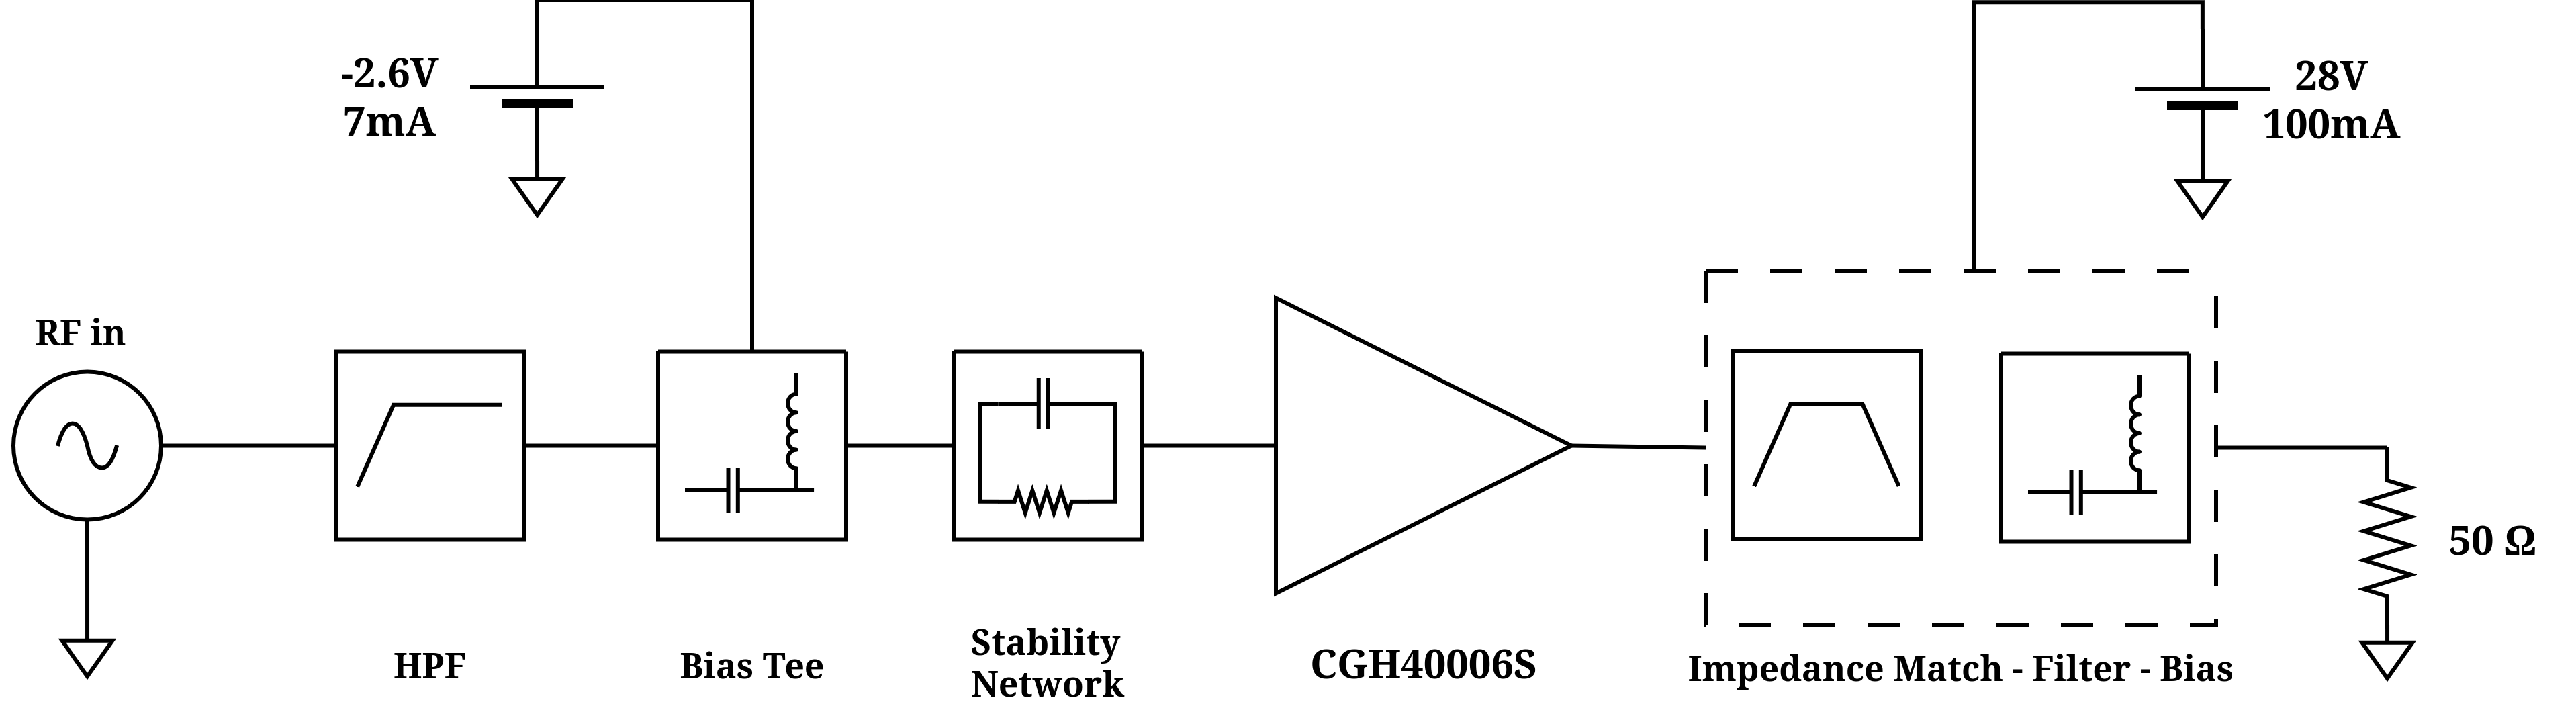
\includegraphics[width=\linewidth]{Figures/07/pa_block_diagram.png}
    \caption{Diagrama en bloques de la topología propuesta para el amplificador de potencia.}
    \label{fig:diagrama_bloques}
\end{figure}

% -----------------------------------------------------------------------------------------------%
\subsection{Diseño esquemático y simulación en ADS}
El proceso de diseño se desarrolló de manera iterativa, comenzando por el análisis de estabilidad del transistor, continuando con la determinación de las impedancias óptimas de carga y de entrada mediante load-pull, y finalizando con el diseño de las redes de adaptación físicas y su verificación con componentes reales.

\textbf{Red de estabilidad.} El primer paso del diseño consistió en evaluar la estabilidad del transistor desnudo, es decir, sin ninguna red adicional de estabilización, en función del punto de polarización. Para ello se armó en ADS el esquemático de la Figura~\ref{fig:pa_ads_stb_bare}, en el cual se polarizó al transistor y se realizó un barrido de la tensión de gate entre -3,5~V y -1,5~V, con $V_{DS}=28$~V fijo, evaluando el factor de estabilidad de Rollett ($K$) entre 0,1 y 6~GHz. Previamente, se validó el modelo del transistor contra la información de la nota de aplicación del fabricante, reproduciendo las curvas características $I_{DS}$-$V_{DS}$ y de transconductancia $G_m$ en función de $V_{GS}$.

\begin{figure}[H]
    \centering
    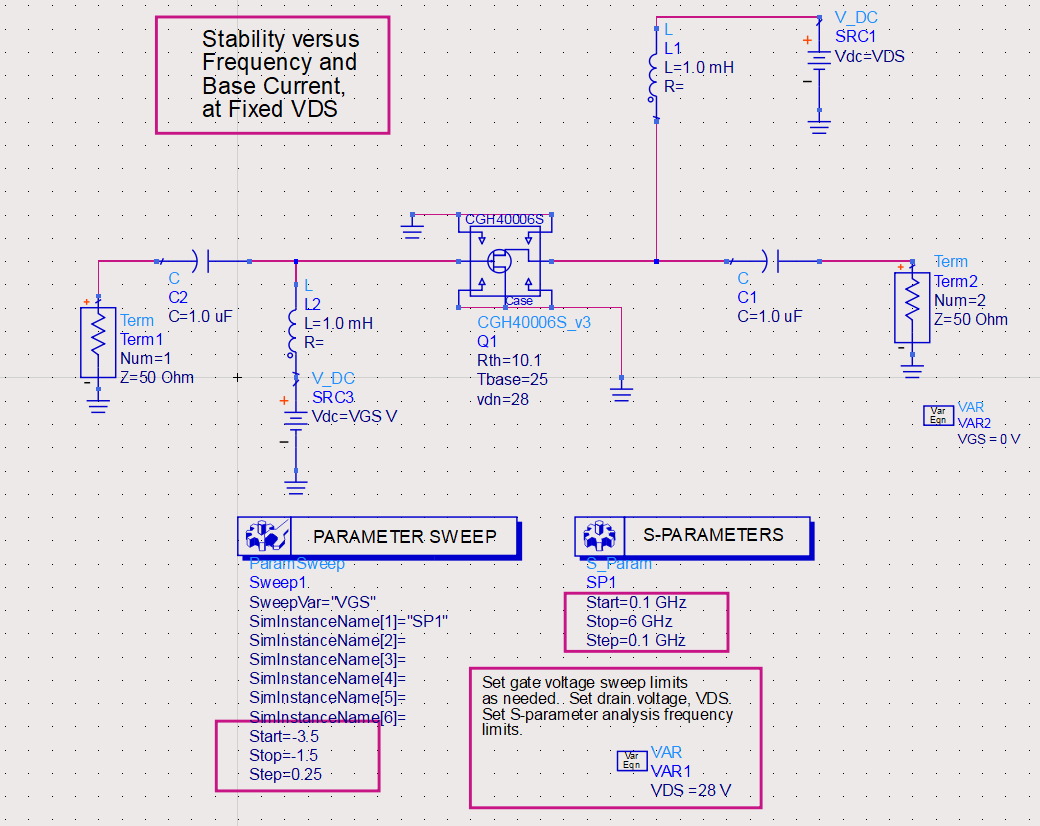
\includegraphics[width=0.7\linewidth]{Figures/07/pa_ads_stb_bare.png}
    \caption{Esquemático empleado para el barrido de estabilidad del transistor en función de la tensión de gate, sin red de estabilidad adicional.}
    \label{fig:pa_ads_stb_bare}
\end{figure}

La Figura~\ref{fig:pa_ads_kfactor_bare} muestra el resultado de este barrido. El caso $V_{GS}=-3,5$~V resulta estable ($K>1$) en toda la banda, pero se trata de un caso trivial, dado que en ese punto el transistor se encuentra en la región de corte y no conduce corriente. Para el resto de los casos, en los que el transistor sí conduce, el factor $K$ mejora a medida que $V_{GS}$ aumenta (se hace menos negativa), estabilizándose a partir de aproximadamente $V_{GS}=-2,5$~V, sin mejoras adicionales significativas por encima de este valor. Aun así, en todos estos casos en los que el transistor conduce, el circuito resulta potencialmente inestable ($K$<1) a bajas frecuencias, lo que evidencia la necesidad de una red de estabilización.

\begin{figure}[H]
    \centering
    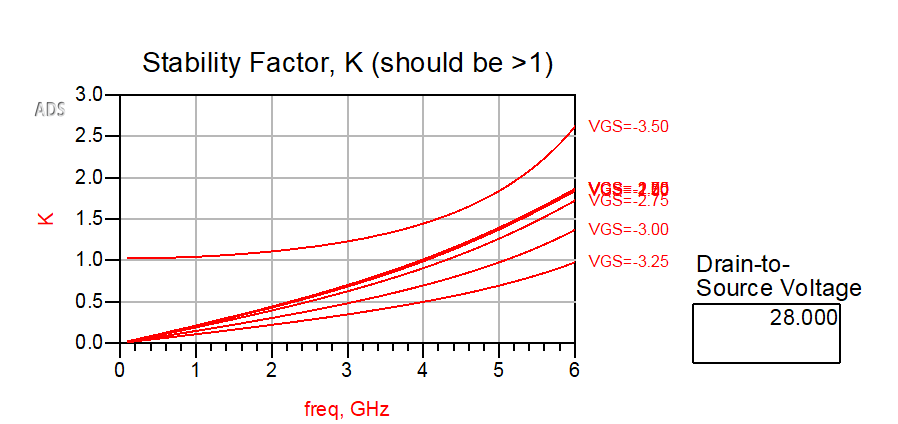
\includegraphics[width=0.8\linewidth]{Figures/07/pa_ads_kfactor_bare.png}
    \caption{Factor de estabilidad de Rollett ($K$) en función de la frecuencia, para distintos valores de $V_{GS}$, sin red de estabilidad adicional.}
    \label{fig:pa_ads_kfactor_bare}
\end{figure}

Se evaluó en primer lugar la incorporación de una resistencia serie de bajo valor en el gate (5, 10 y 50~$\Omega$) como única medida de estabilización, la cual no resultó suficiente para lograr estabilidad incondicional en ninguno de los tres casos. Siguiendo el criterio de diseño de la nota de aplicación del fabricante \cite{macom2023an}, reproducido en la Figura~\ref{fig:pa_an_stb_net}, se incorporó adicionalmente una red de realimentación resistivo-capacitiva entre drain y gate ($R=432\,\Omega$, $C=82$~pF), en conjunto con la resistencia serie de gate ($R=5\,\Omega$), conformando el esquemático de la Figura~\ref{fig:pa_ads_stb_sch_v1}.

\begin{figure}[H]
    \centering
    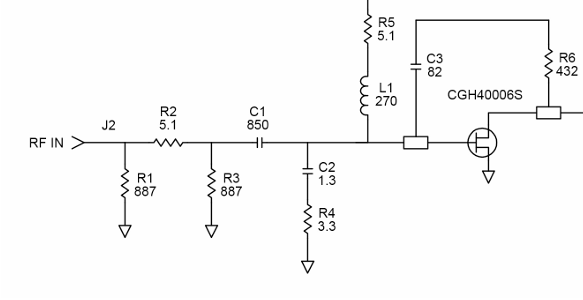
\includegraphics[width=0.8\linewidth]{Figures/07/pa_an_stb_net.png}
    \caption{Red de estabilidad de referencia propuesta en la nota de aplicación del fabricante del transistor \cite{macom2023an}.}
    \label{fig:pa_an_stb_net}
\end{figure}

\begin{figure}[H]
    \centering
    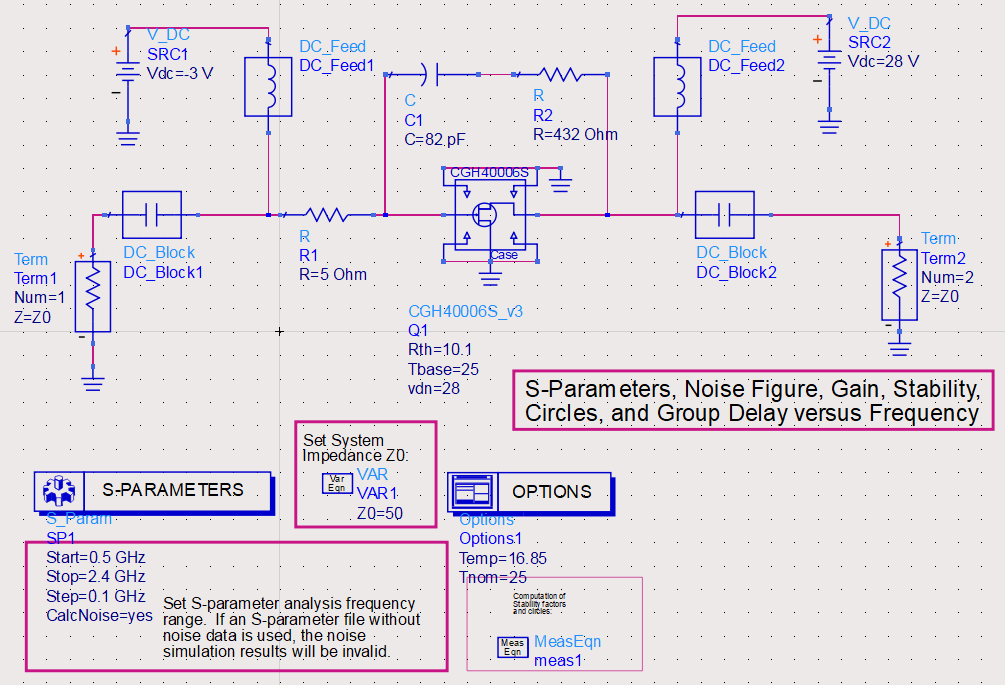
\includegraphics[width=\linewidth]{Figures/07/pa_ads_stb_sch_v1.png}
    \caption{Esquemático de la primera red de estabilidad implementada en ADS, con resistencia serie de gate y realimentación resistivo-capacitiva entre drain y gate.}
    \label{fig:pa_ads_stb_sch_v1}
\end{figure}

Con esta red incorporada, se evaluó la estabilidad incondicional del circuito mediante los factores $\mu_{load}$ y $\mu_{source}$, cuyo resultado se presenta en la Figura~\ref{fig:pa_ads_mu_v1}. Ambos factores resultaron mayores a la unidad en la totalidad de la banda simulada (0 a 6~GHz) y para todos los puntos de polarización evaluados, confirmando la estabilidad incondicional del circuito. Esta conclusión se verificó adicionalmente mediante una simulación de adaptación simultánea, ruido y círculos de estabilidad, cuyo resultado se muestra en la Figura~\ref{fig:pa_ads_stbcircles_v1}: la ausencia de círculos de inestabilidad de carga dentro del diagrama de Smith indica que, para el punto de polarización analizado, el circuito resulta estable frente a cualquier condición de carga posible.

\begin{figure}[H]
    \centering
    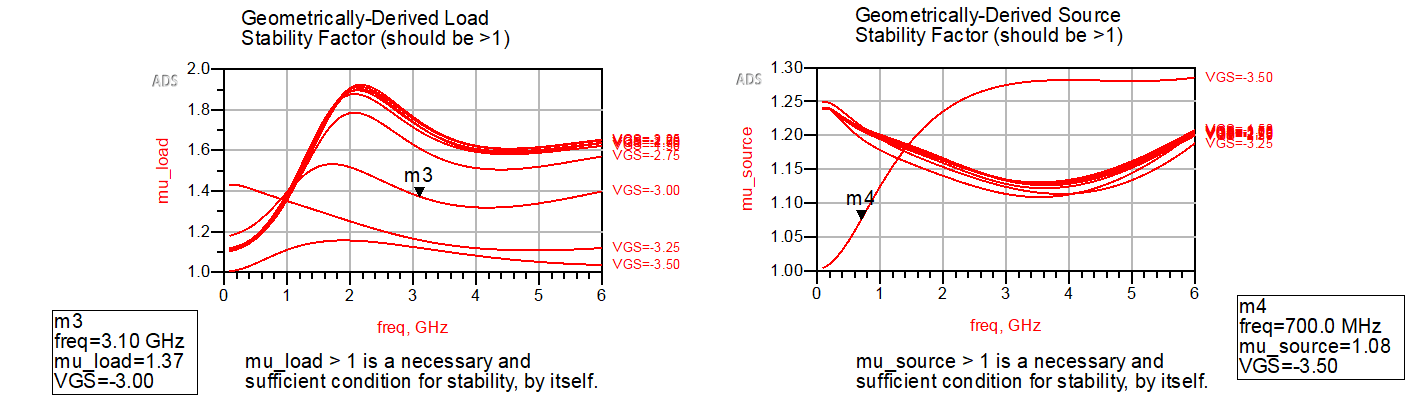
\includegraphics[width=\linewidth]{Figures/07/pa_ads_mu_v1.png}
    \caption{Factores de estabilidad de carga ($\mu_{load}$) y de fuente ($\mu_{source}$) en función de la frecuencia, para la primera red de estabilidad implementada.}
    \label{fig:pa_ads_mu_v1}
\end{figure}

\begin{figure}[H]
    \centering
    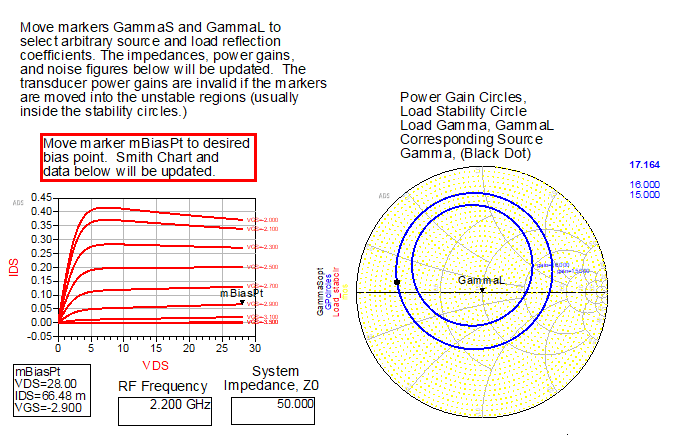
\includegraphics[width=0.7\linewidth]{Figures/07/pa_ads_stbcircles_v1.png}
    \caption{Círculos de ganancia de potencia y de estabilidad de carga en el diagrama de Smith, sin círculos de inestabilidad presentes dentro de la región de interés, confirmando estabilidad incondicional.}
    \label{fig:pa_ads_stbcircles_v1}
\end{figure}

A continuación fue llevada a cabo una simulación de load-pull para determinar las impedancias de carga y de fuente ($\Gamma_L$ y $\Gamma_S$) del transistor. Sin embargo, este análisis no contemplaba la línea de transmisión física necesaria para conectar la resistencia y el capacitor de la red de estabilidad. Al avanzar hacia el diseño físico e incorporar dicha línea, se identificó que esta introducía una fase adicional que volvía inestable al circuito, a pesar de que la red discreta ideal garantizaba estabilidad incondicional. Este hallazgo obligó a rediseñar la red de estabilidad teniendo en cuenta explícitamente el efecto de la línea de transmisión, hasta recuperar la condición de estabilidad incondicional.

Dado que este rediseño modificaba las condiciones de carga y de fuente vistas por el transistor, fue necesario repetir el load-pull para obtener nuevos valores de $\Gamma_L$ y $\Gamma_S$ consistentes con la red de estabilidad ya corregida. Al evaluar esta nueva solución se observó que la resistencia de la red de estabilidad disipaba aproximadamente 1~W, por lo que, en lugar de continuar iterando sobre el mismo criterio, se optó por cambiar la estrategia de diseño, abandonando la búsqueda de estabilidad incondicional en favor de un diseño condicionalmente estable, es decir, estable para el mayor rango posible de condiciones de carga y de fuente, pero no necesariamente para la totalidad del diagrama de Smith. Esta decisión se fundamenta en que garantizar estabilidad incondicional compromete de manera significativa la ganancia, la eficiencia y la potencia de salida del amplificador, mientras que una solución condicionalmente estable, correctamente delimitada, permite recuperar gran parte de estas prestaciones a cambio de restringir el diseño de la red de adaptación a una región acotada del diagrama de Smith.

El nuevo diseño de la red de estabilidad se basó en \cite{bahl2009}, consistiendo esta en un circuito RC paralelo ($R=25~\Omega, C=5~pF$) en el gate del transistor, como se observa en la Figura~\ref{fig:pa_ads_stb_sch_v2}. Ante este nuevo diseño, el análisis de $\mu_{load}$ en función de la frecuencia y del punto de polarización fue repetido, el cual se presenta en la Figura~\ref{fig:pa_ads_mu_v2}. A diferencia del caso incondicionalmente estable de la Figura~\ref{fig:pa_ads_mu_v1}, en este caso $\mu_{load}$ se hace menor a la unidad a partir de aproximadamente 700~MHz para la polarización nominal ($V_{GS}=-3$\,~V), lo cual es esperable y aceptable dado el nuevo criterio de diseño adoptado. Al elevar ligeramente el punto de polarización hacia la región de Clase AB ($V_{GS}=-2,75$\,~V), este cruce se desplaza hasta aproximadamente 500~MHz, lo que evidencia que el punto de polarización constituye una variable de la cual depende el margen de estabilidad.

\begin{figure}[H]
    \centering
    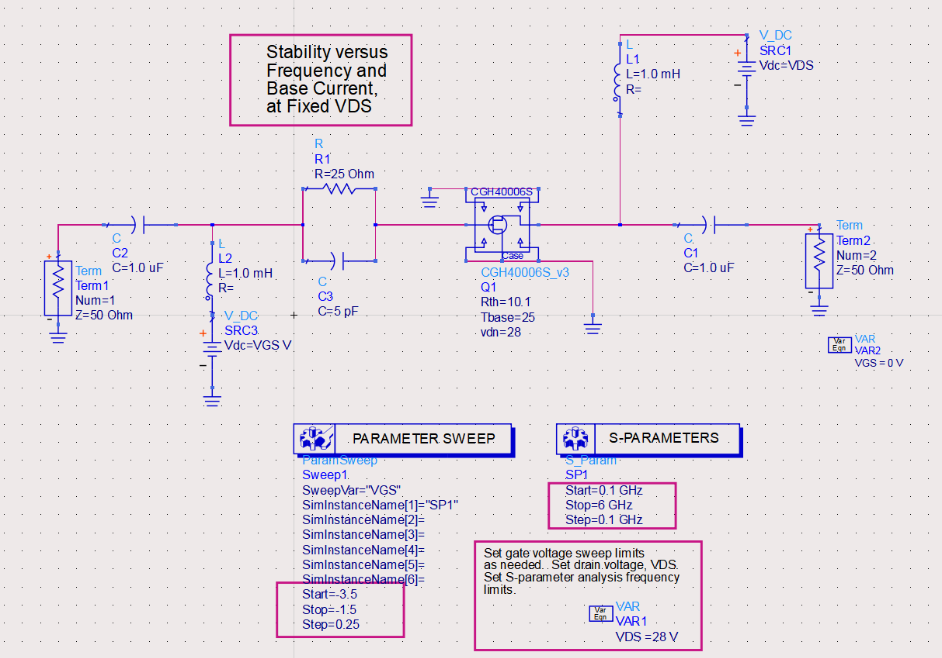
\includegraphics[width=\linewidth]{Figures/07/pa_ads_stb_sch_v2.png}
    \caption{Esquemático de la segunda red de estabilidad implementada en ADS con circuito RC paralelo en serie al gate del transistor.}
    \label{fig:pa_ads_stb_sch_v2}
\end{figure}

\begin{figure}[H]
    \centering
    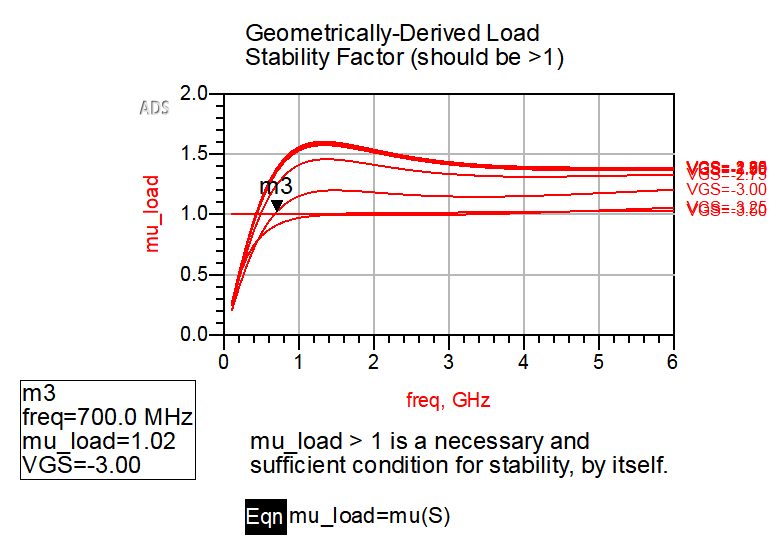
\includegraphics[width=0.8\linewidth]{Figures/07/pa_ads_mu_v2.png}
    \caption{Factor de estabilidad de carga ($\mu_{load}$) en función de la frecuencia, para la red de estabilidad condicionalmente estable, en distintos puntos de polarización de gate.}
    \label{fig:pa_ads_mu_v2}
\end{figure}

A partir de este análisis se identificaron dos frecuencias críticas para el diseño de la red de adaptación. La primera, de 700~MHz, corresponde al punto en el que el circuito comienza a presentar una región de inestabilidad. La segunda, de 350~MHz, se vincula con la longitud de onda guiada de aproximadamente 40~cm, dado que una línea de transmisión deja de comportarse como tal, y pasa a comportarse aproximadamente como un conductor que refleja directamente la impedancia de su terminación, cuando su longitud resulta inferior a $\lambda/10$, es decir, inferior a 4~cm para esta frecuencia. En consecuencia, el objetivo de diseño de la red de adaptación se estableció en presentar la menor desadaptación posible por debajo de 700~MHz, evitando que el coeficiente de reflexión visto por el transistor ingrese en la región delimitada por el círculo de inestabilidad de carga en ese rango.

Los círculos de estabilidad se evaluaron en los puntos críticos de 500~MHz y 300~MHz para la polarización nominal, obteniéndose módulos de coeficiente de reflexión límite de 0,841 y 0,566 respectivamente, por debajo de los cuales el circuito permanece estable frente a cualquier condición de carga. Al repetir este análisis para el punto de polarización de Clase AB ($V_{GS}=-2,8$~V) en 300~MHz, el módulo del coeficiente de reflexión límite se incrementó a 0,684, una mejora relativa de aproximadamente el 20\,\% en el radio de la región de cargas admisibles, confirmando nuevamente el efecto beneficioso de operar levemente por encima de la polarización de Clase B estricta sobre el margen de estabilidad del circuito.

\begin{figure}[H]
    \centering
    \begin{subfigure}{0.48\linewidth}
        \centering
        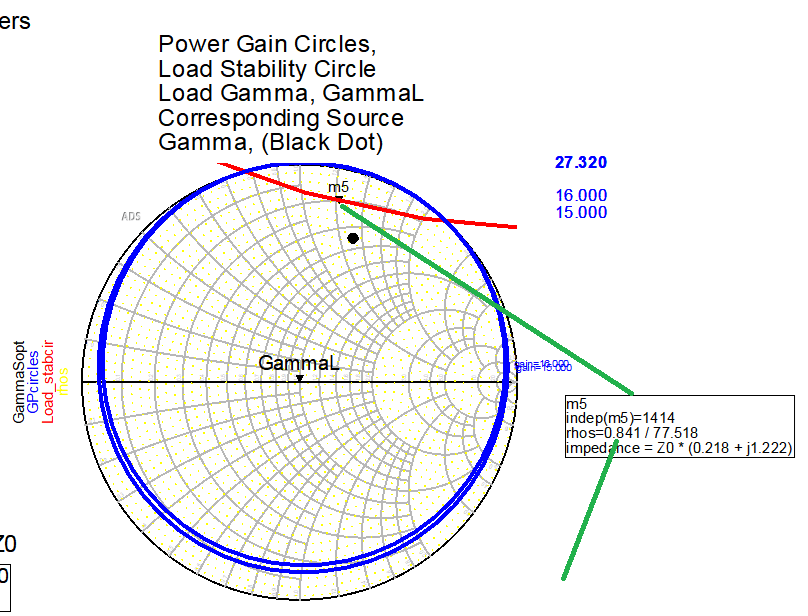
\includegraphics[width=\linewidth]{Figures/07/pa_circulo_500mhz.png}
        \caption{500\,MHz, $V_{GS}=-3$~V ($|\Gamma|=0,841$)}
    \end{subfigure}
    \hfill
    \begin{subfigure}{0.48\linewidth}
        \centering
        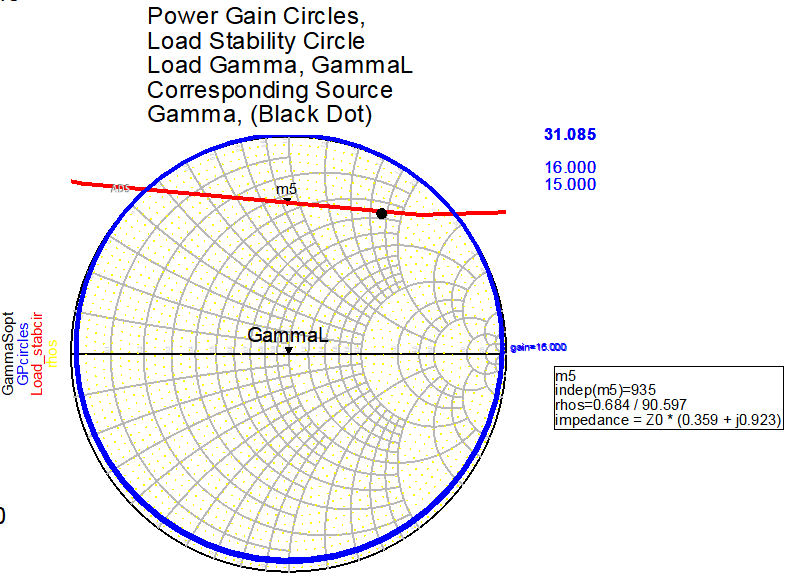
\includegraphics[width=\linewidth]{Figures/07/pa_circulo_300mhz_ab.png}
        \caption{300\,MHz, $V_{GS}=-2,8$~V ($|\Gamma|=0,684$)}
    \end{subfigure}
    \caption{Círculos de estabilidad de carga en el plano de Smith, mostrando el coeficiente de reflexión límite $\rho$ para distintas frecuencias y puntos de polarización.}
    \label{fig:pa_circulos_estabilidad}
\end{figure}

Con el circuito ya prácticamente terminado, y en paralelo con la selección de los componentes reales descripta más adelante, se revisó nuevamente la red de estabilidad, incorporando un nuevo juego de resistencias dispuesto para aumentar simultáneamente la conductancia en paralelo y la resistencia en serie vistas por el transistor. Esta última revisión, presentada en la Figura~\ref{fig:pa_ads_final}, logró nuevamente estabilidad incondicional del circuito, a costa de una pérdida de ganancia que resultó mínima y despreciable frente al beneficio de eliminar el riesgo de oscilaciones no deseadas. En el esquemático puede observarse que las resistencias R3 y R5 incorporan cada una un inductor en serie (L8 y L7 respectivamente), los cuales no forman parte del diseño original de la red sino que modelan la inductancia parásita propia de las resistencias reales seleccionadas, cuyo efecto sobre el desempeño del circuito se analiza en la Sección~\ref{sec:resultados}.

\begin{figure}[H]
    \centering
    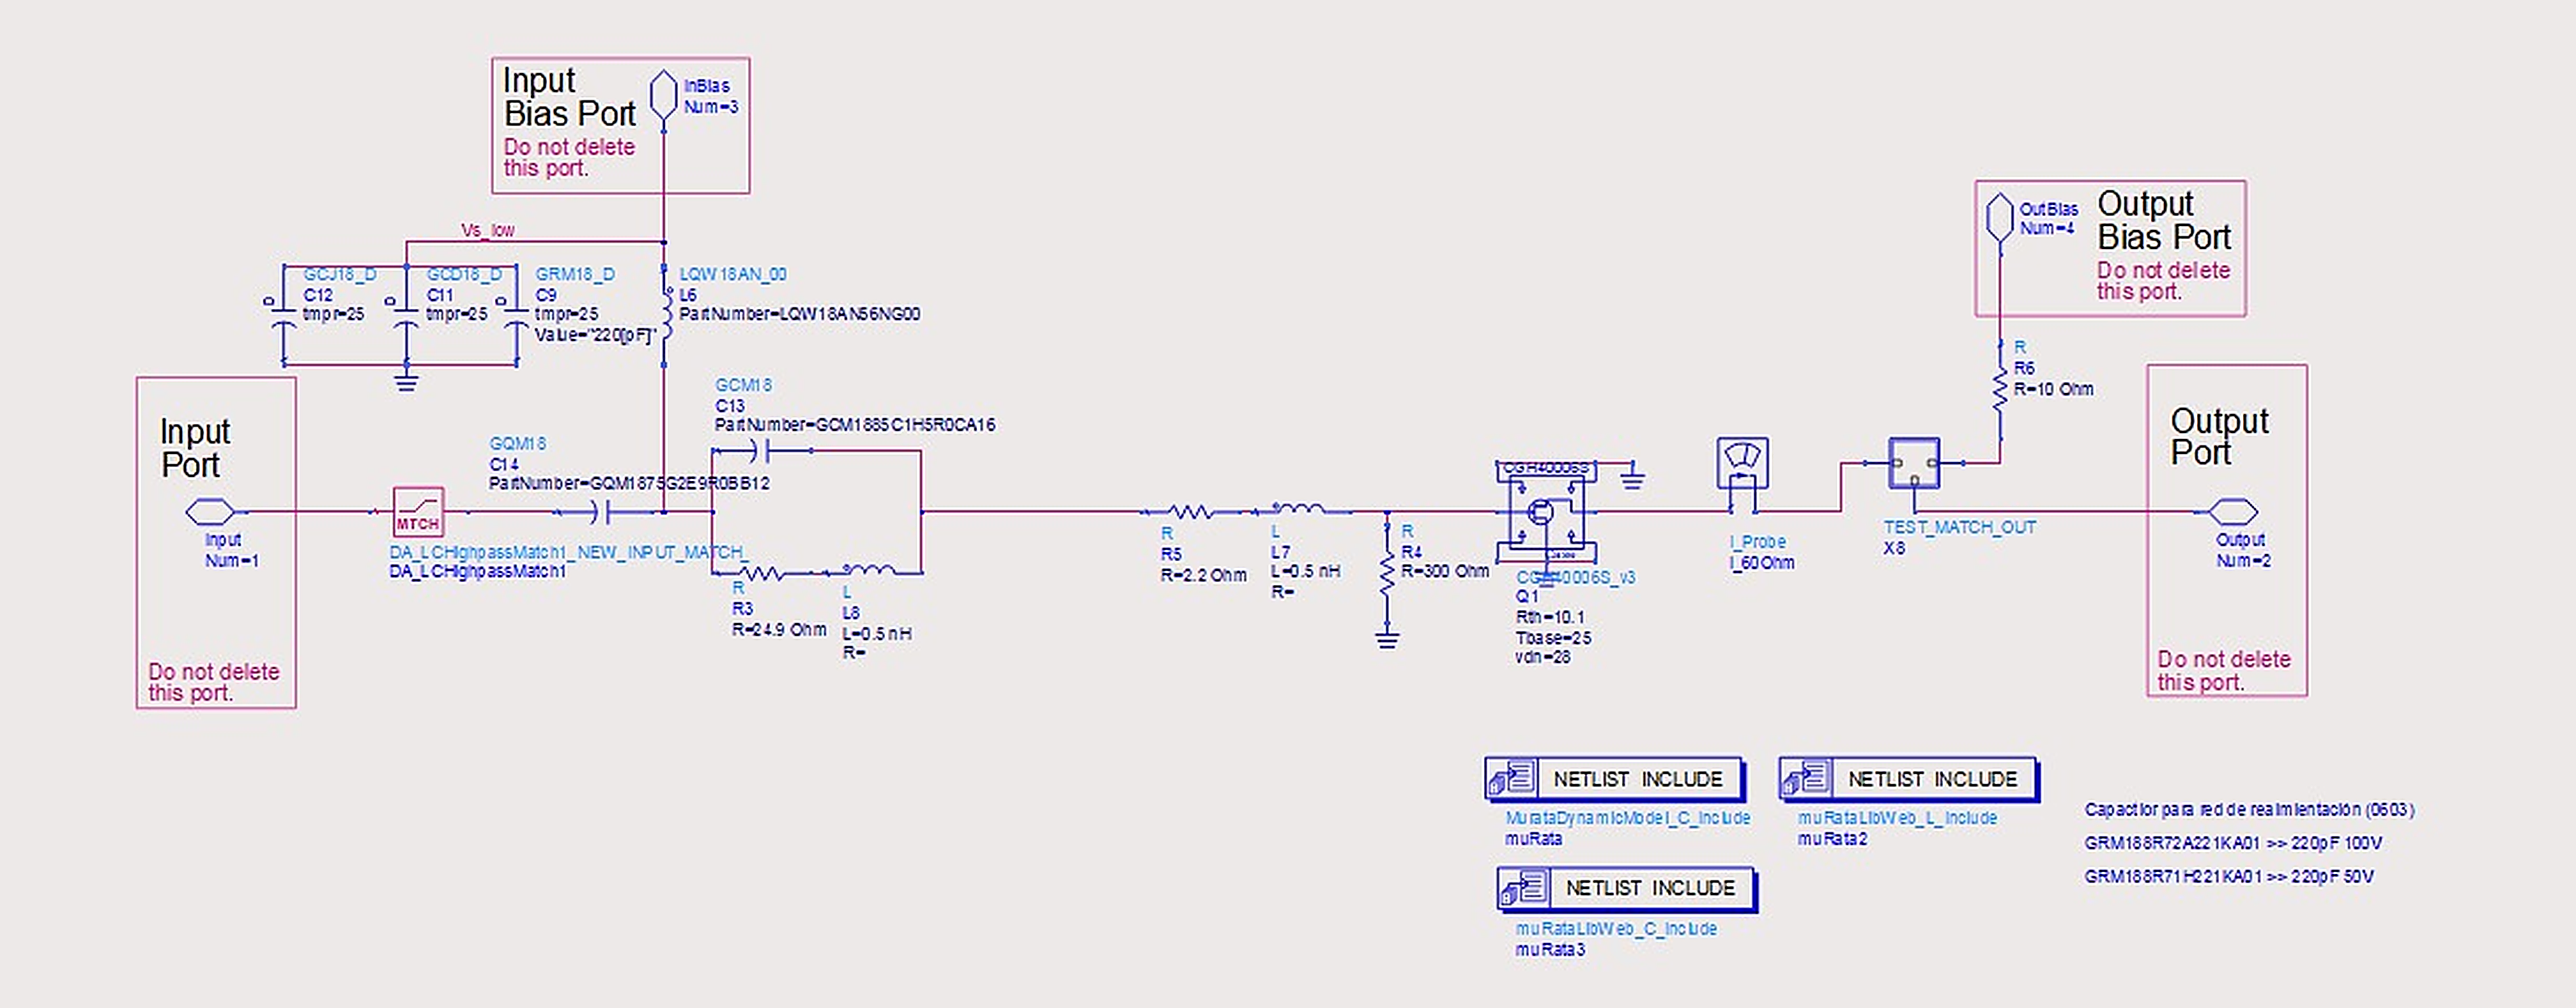
\includegraphics[width=\linewidth]{Figures/07/pa_ads_final.png}
    \caption{Esquemático de la red de estabilidad final, incorporada con el circuito ya prácticamente terminado, incluyendo los inductores parásitos (L7, L8) asociados a las resistencias reales de la red.}
    \label{fig:pa_ads_final}
\end{figure}

La Figura~\ref{fig:pa_ads_stability_plot} confirma el resultado de esta última revisión: tanto $\mu_{load}$ como $\mu_{source}$ se mantienen por encima de la unidad en la totalidad de la banda simulada (0,5 a 8~GHz), verificando la estabilidad incondicional del circuito final.

\begin{figure}[H]
    \centering
    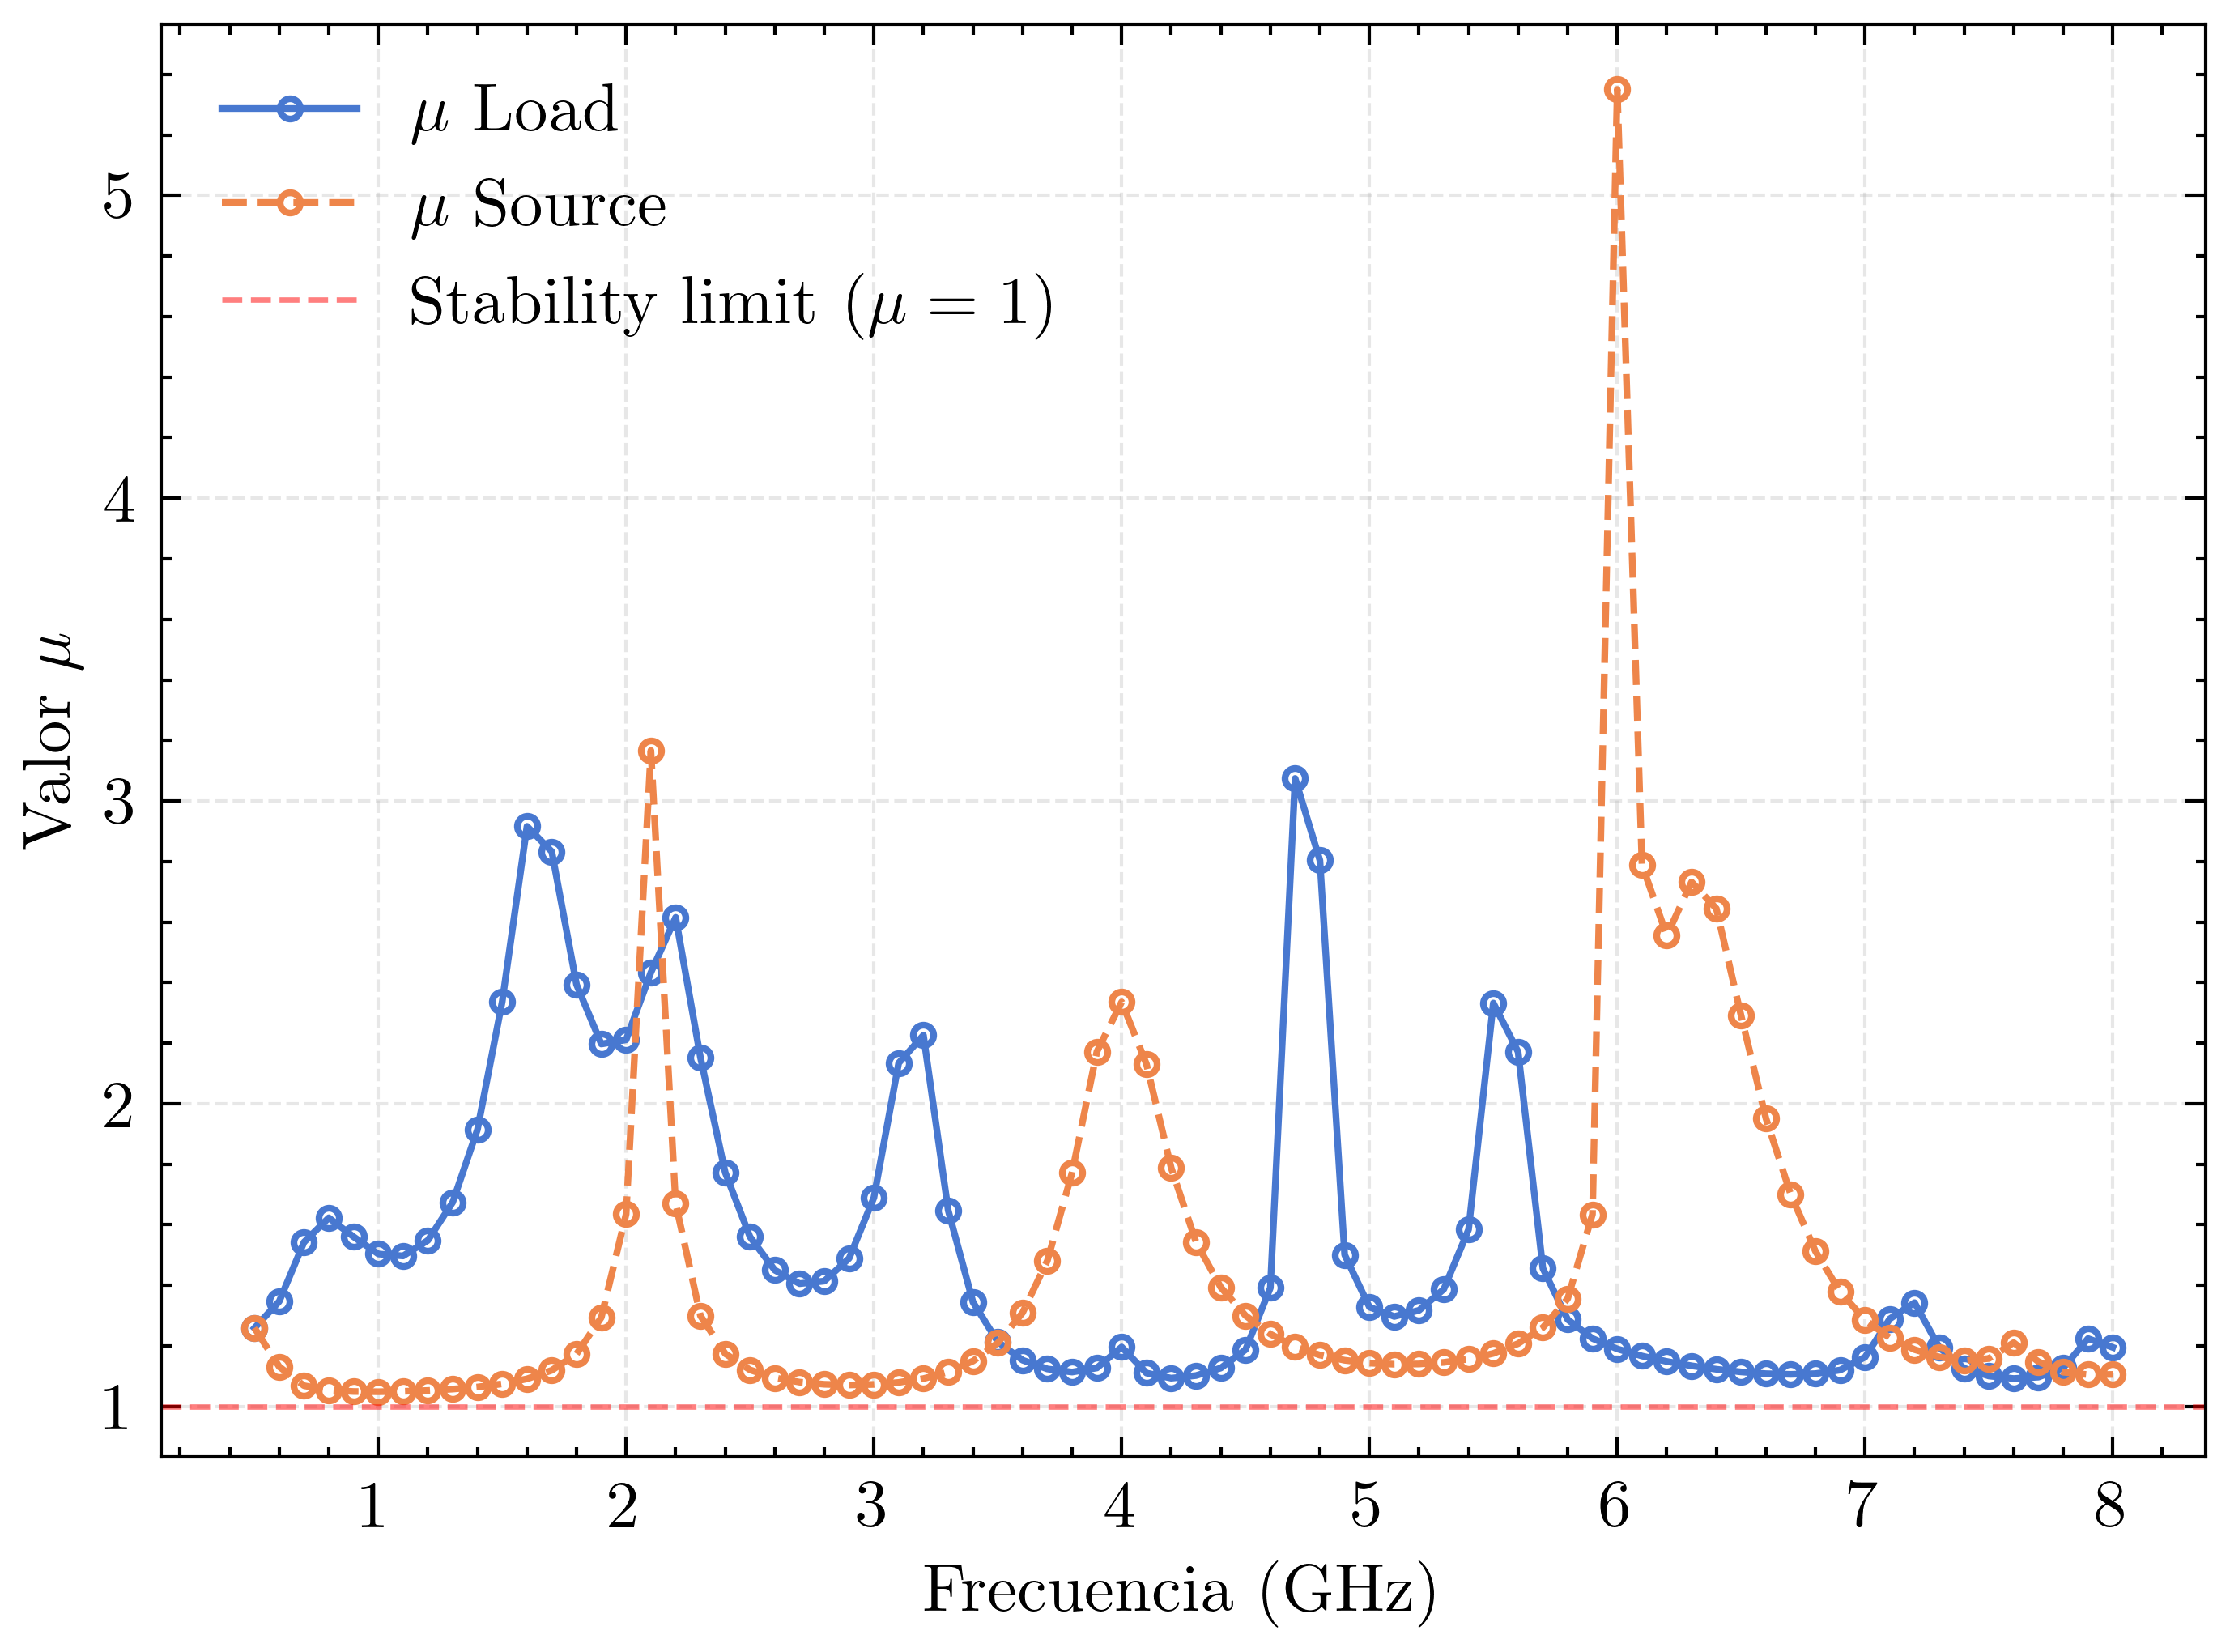
\includegraphics[width=0.6\linewidth]{Figures/07/pa_stability_plot.png}
    \caption{Factores de estabilidad $\mu_{load}$ y $\mu_{source}$ en función de la frecuencia, correspondientes a la red de estabilidad final del amplificador.}
    \label{fig:pa_ads_stability_plot}
\end{figure}

\textbf{Simulación de load-pull.} Una vez definida la red de estabilidad, se determinó la impedancia de carga que maximiza el desempeño de gran señal del transistor mediante load-pull. Con el objetivo de aislar el comportamiento del transistor de los elementos de la red de salida durante esta caracterización, el circuito de load-pull se armó de manera tal que la carga barrida se conectara directamente a los puertos del transistor, sin la influencia de las líneas de transmisión ni los capacitores que posteriormente conformarían la red de adaptación física. El valor de la impedancia de carga seleccionado fue de $Z_L=(24.1 + j52) \,\Omega$. La Figura~\ref{fig:pa_loadpull} ilustra el diagrama de Smith con los contornos obtenidos mediante load-pull.

\begin{figure}[H]
    \centering
    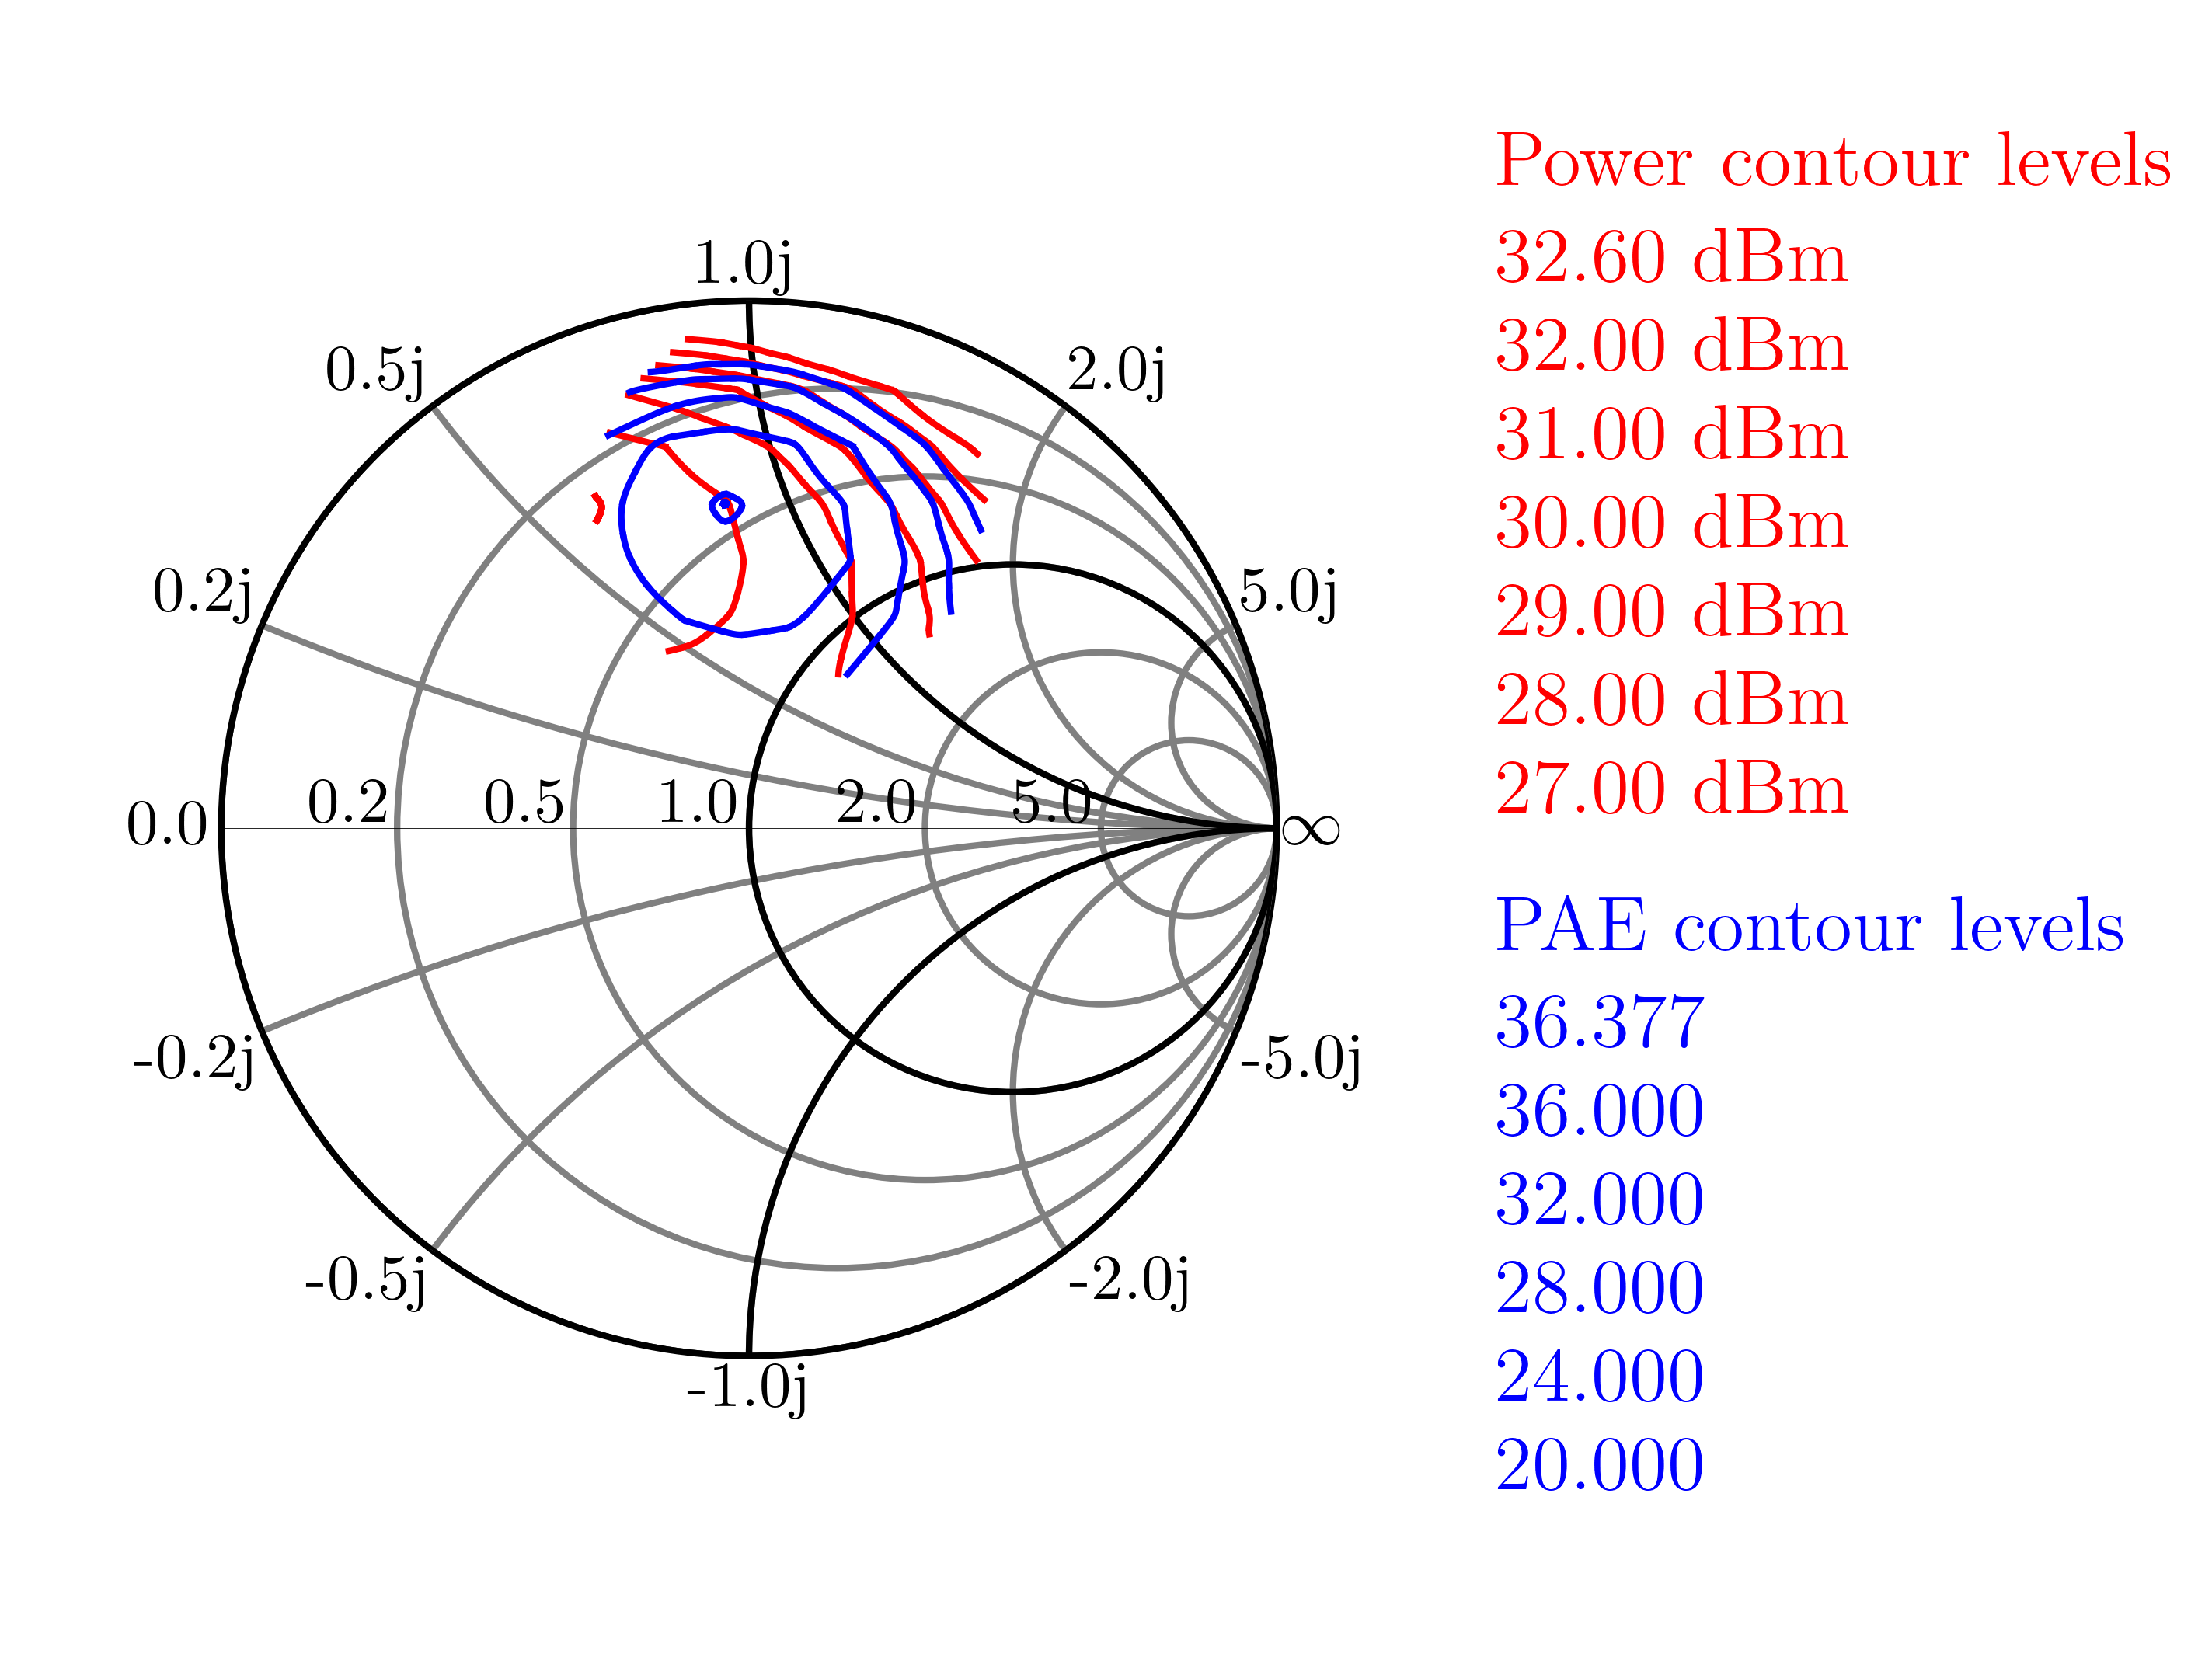
\includegraphics[width=0.9\linewidth]{Figures/07/pa_loadpull_plot.png}
    \caption{Contornos de potencia entregada y de PAE obtenidos mediante simulación de load-pull.}
    \label{fig:pa_loadpull}
\end{figure}

Durante las primeras pruebas de load-pull, con el primer diseño de la red de estabilidad, se evaluó el efecto de reducir la potencia de excitación de entrada manteniendo fija la impedancia de carga. Al reducir la potencia de entrada, el punto de operación se desplaza dentro de la misma región de máxima ganancia y máxima eficiencia de los contornos de load-pull, aunque con una eficiencia de potencia añadida menor. Concretamente, al reducir la potencia de salida de 3~W a 2~W la eficiencia cae de aproximadamente 44\,\% a 37\,\%, sin embargo, la potencia continua que debe entregar la fuente de alimentación resulta proporcionalmente menor, de acuerdo con la relación:

\begin{equation}
    P_{fuente} = \frac{P_{out}}{\eta}
    \label{eq:potencia_fuente}
\end{equation}

lo que arroja $P_{fuente}(P_{out}=3~\,W) \approx 6,81~\,W$ frente a $P_{fuente}(P_{out}=2~\,W) \approx 5,40~\,W$. Esta observación resulta relevante para una aplicación satelital con presupuesto energético acotado, dado que evidencia que, para una misma impedancia de carga, la elección del nivel de excitación de entrada permite priorizar entre maximizar la eficiencia o minimizar la potencia total consumida de la plataforma, según el criterio de diseño que se desee adoptar.

\textbf{Selección de componentes reales y resonancias parásitas.} Sobre la base del diseño obtenido con componentes ideales, se reemplazaron los capacitores e inductores discretos por sus modelos reales de montaje superficial, provenientes de la biblioteca del fabricante muRata, empleando la biblioteca dinámica para los capacitores y la biblioteca estática para los inductores. Este reemplazo reveló que el comportamiento de dichos componentes se veía afectado por sus inductancias parásitas, las cuales provocaban resonancias en frecuencias cercanas a la de operación, e incluso por debajo de esta, con impacto directo sobre la confiabilidad del circuito: los parámetros resultantes eran muy sensibles a pequeñas variaciones tanto en la longitud de las líneas de transmisión como en los valores de los componentes, además de degradar la estabilidad y la ganancia del amplificador.

Para resolver este problema se buscaron componentes pasivos reales mediante la herramienta SimSurfing del fabricante muRata, seleccionando capacitores e inductores cuya frecuencia de autorresonancia no se encontrara próxima a la banda de operación de interés, y verificando adicionalmente su disponibilidad en stock en los proveedores Digikey y JLCPCB. Los criterios adoptados para la selección de cada componente fueron el tamaño del encapsulado (0603 o 0805), el valor nominal, la tolerancia y los valores máximos admisibles de tensión, en el caso de los capacitores, y de corriente, en el caso de los inductores.

Una vez incorporados los componentes reales seleccionados de esta manera, el circuito resultó considerablemente más robusto frente a variaciones. Durante las pruebas en el segundo diseño de la red de estabilidad, la resimulación del circuito con componentes reales resultó en una perdida de 0.4\,W respecto del diseño ideal, mientras que la eficiencia se mantuvo en un nivel similar. Adicionalmente, se observó que para un mismo tipo de componente, cuanto mayor es el encapsulado, mayores resultan los valores de sus elementos parásitos. La utilización de componentes reales puede observarse en la Figura~\ref{fig:pa_ads_final}, donde inductores y capacitores reales tienen asignado su respectivo número de parte.

\textbf{Diseño de la red de adaptación de salida.} El diseño físico de la red de adaptación de salida se inició empleando líneas de transmisión ideales, incorporando dos consideraciones particulares de diseño. En primer lugar, en lugar de emplear un inductor de choque para aislar la fuente de alimentación de la señal de radiofrecuencia, esta función se cumple mediante una línea de transmisión de 50~$\Omega$ de aproximadamente $90^\circ$ eléctricos (es decir, de longitud $\lambda/4$), la cual refleja hacia el resto de la red la baja impedancia de la fuente de alimentación como un circuito abierto en el nodo de interés a la frecuencia de operación. En segundo lugar, se incorporaron stubs en la red, dispuestos con el objetivo de presentar una impedancia de cortocircuito en las frecuencias armónicas de la señal, contribuyendo a suprimir el contenido espectral no deseado a la salida del amplificador. Posteriormente se agregaron capacitores discretos de montaje superficial, cumpliendo la función de filtros de fuente de DC y como filtro de continua sobre la línea de RF. 

\begin{figure}[H]
    \centering
    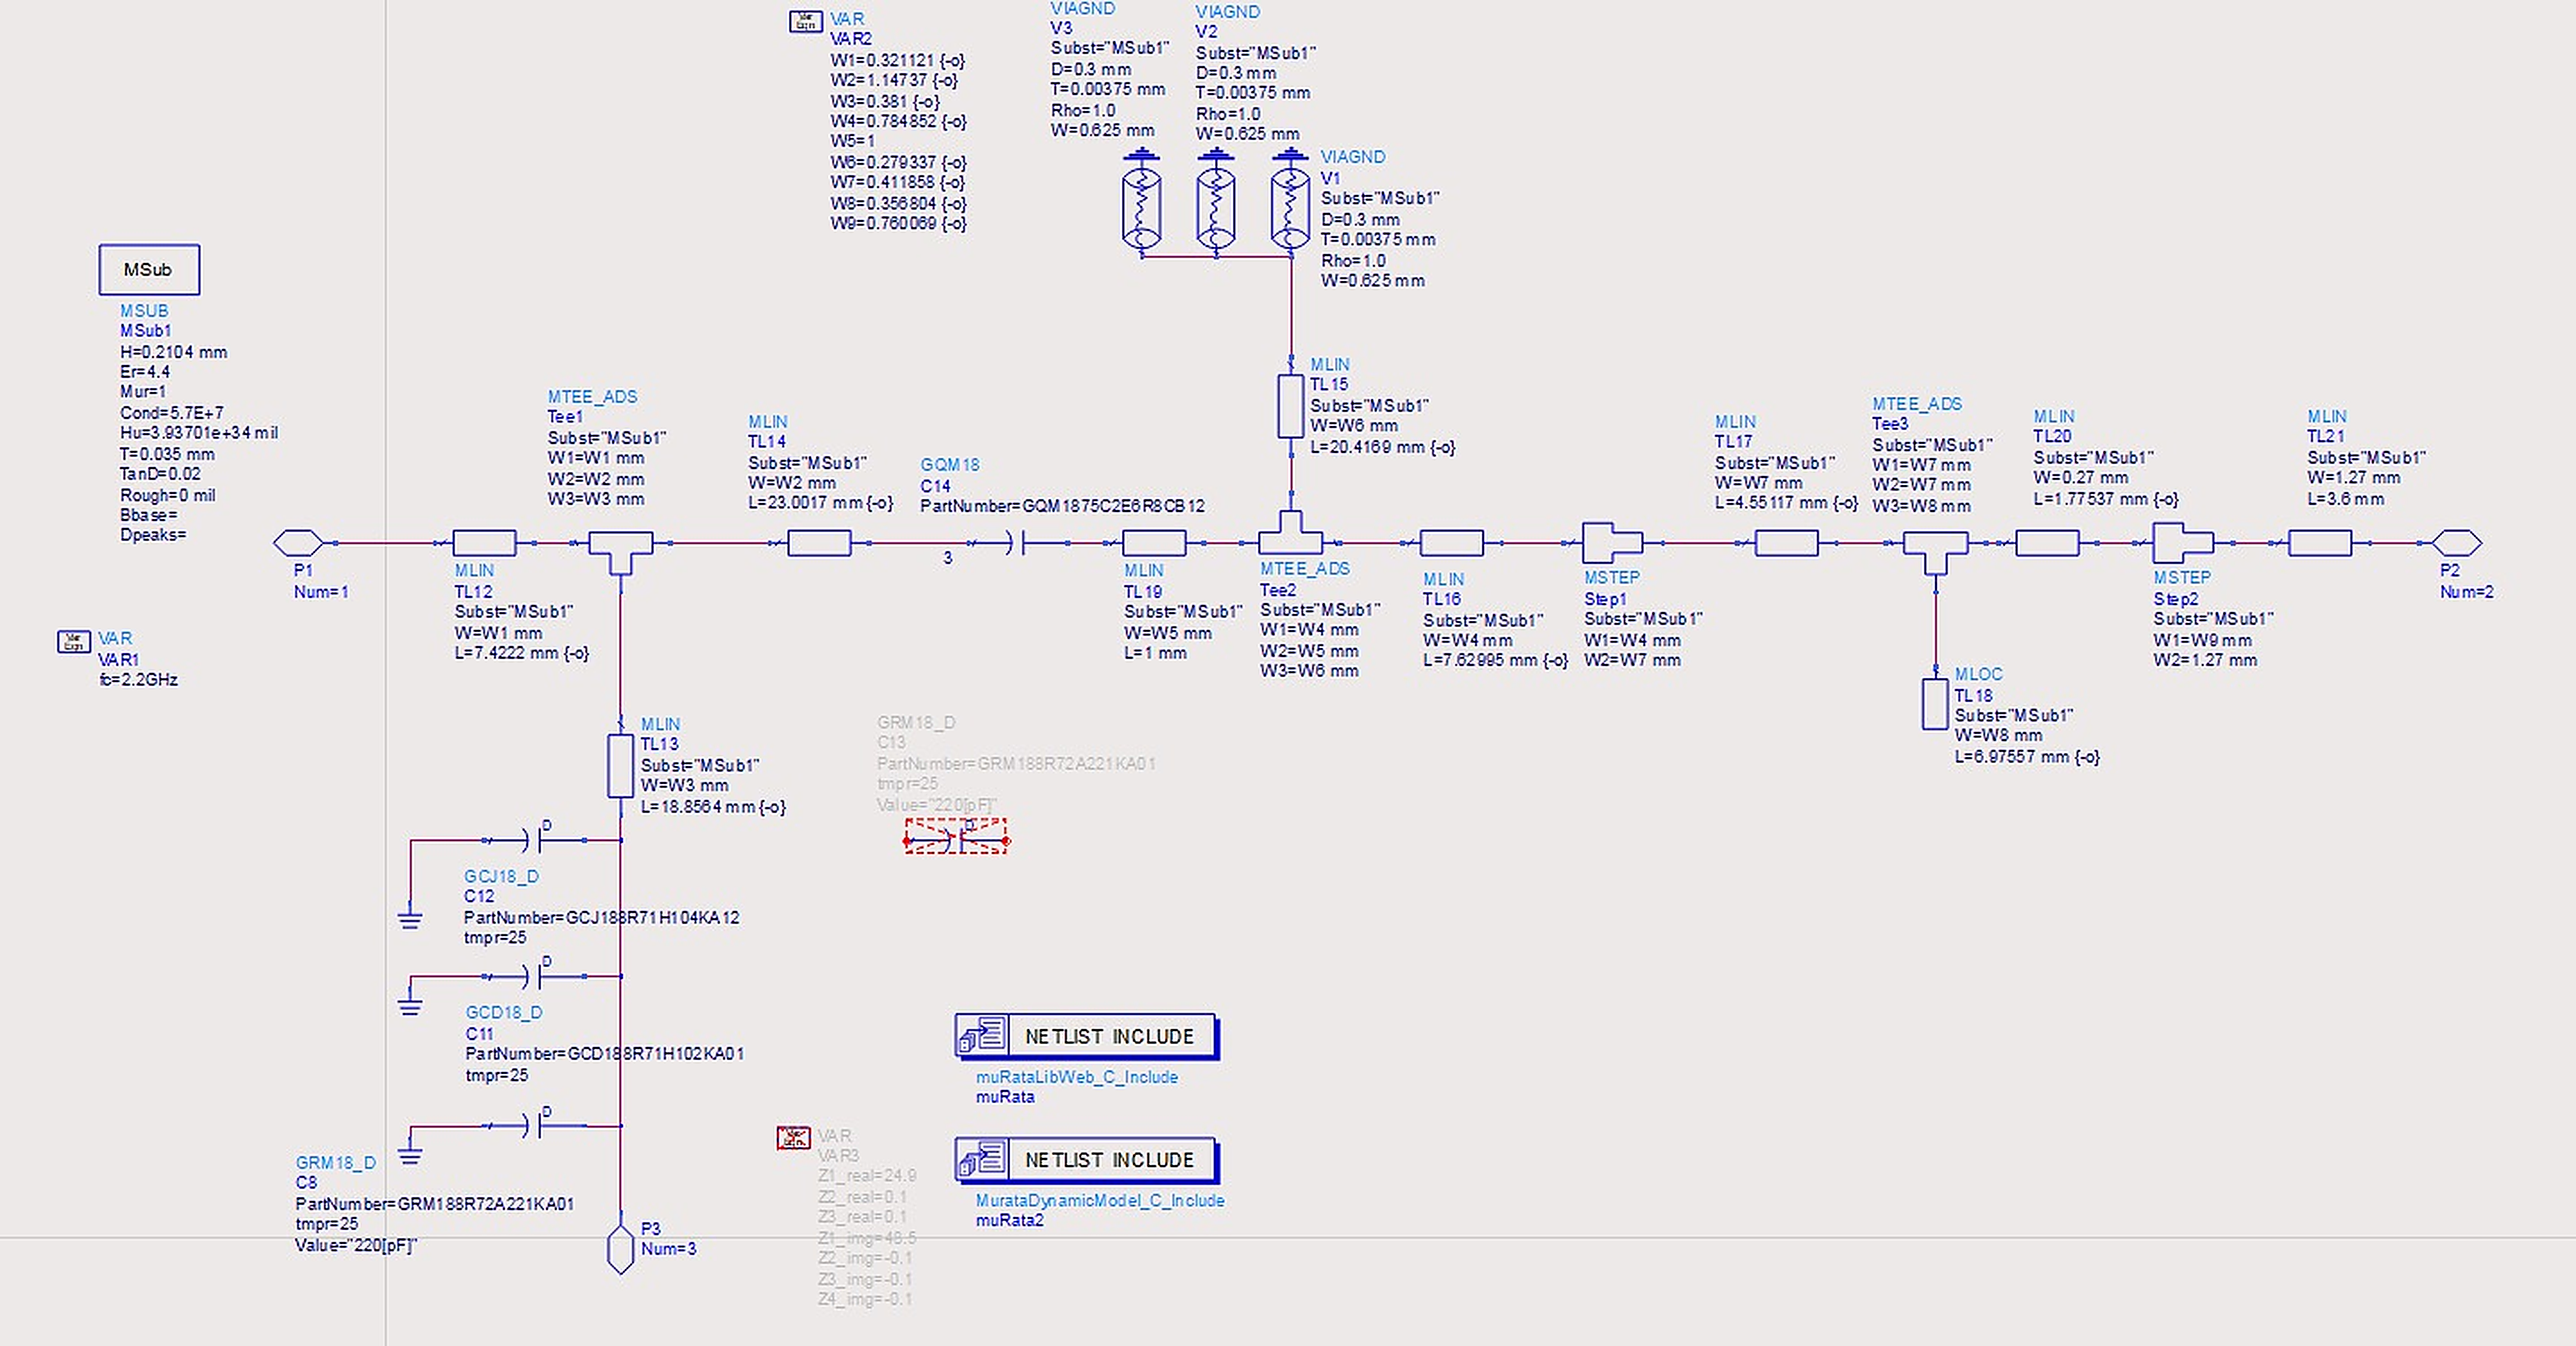
\includegraphics[width=\linewidth]{Figures/07/pa_ads_out_match.png}
    \caption{Circuito de adaptación de salida del diseño final del amplificador de potencia.}
    \label{fig:pa_match_out}
\end{figure}

\textbf{Diseño de la red de adaptación de entrada.} De manera análoga a la red de salida, el diseño físico de la red de adaptación de entrada se realizó con líneas de transmisión ideales complementadas con componentes discretos reales. La Figura~\ref{fig:pa_match_in} muestra el esquemático resultante, la cual además de adaptar, cumple la función de filtro pasa altos.

\begin{figure}[H]
    \centering
    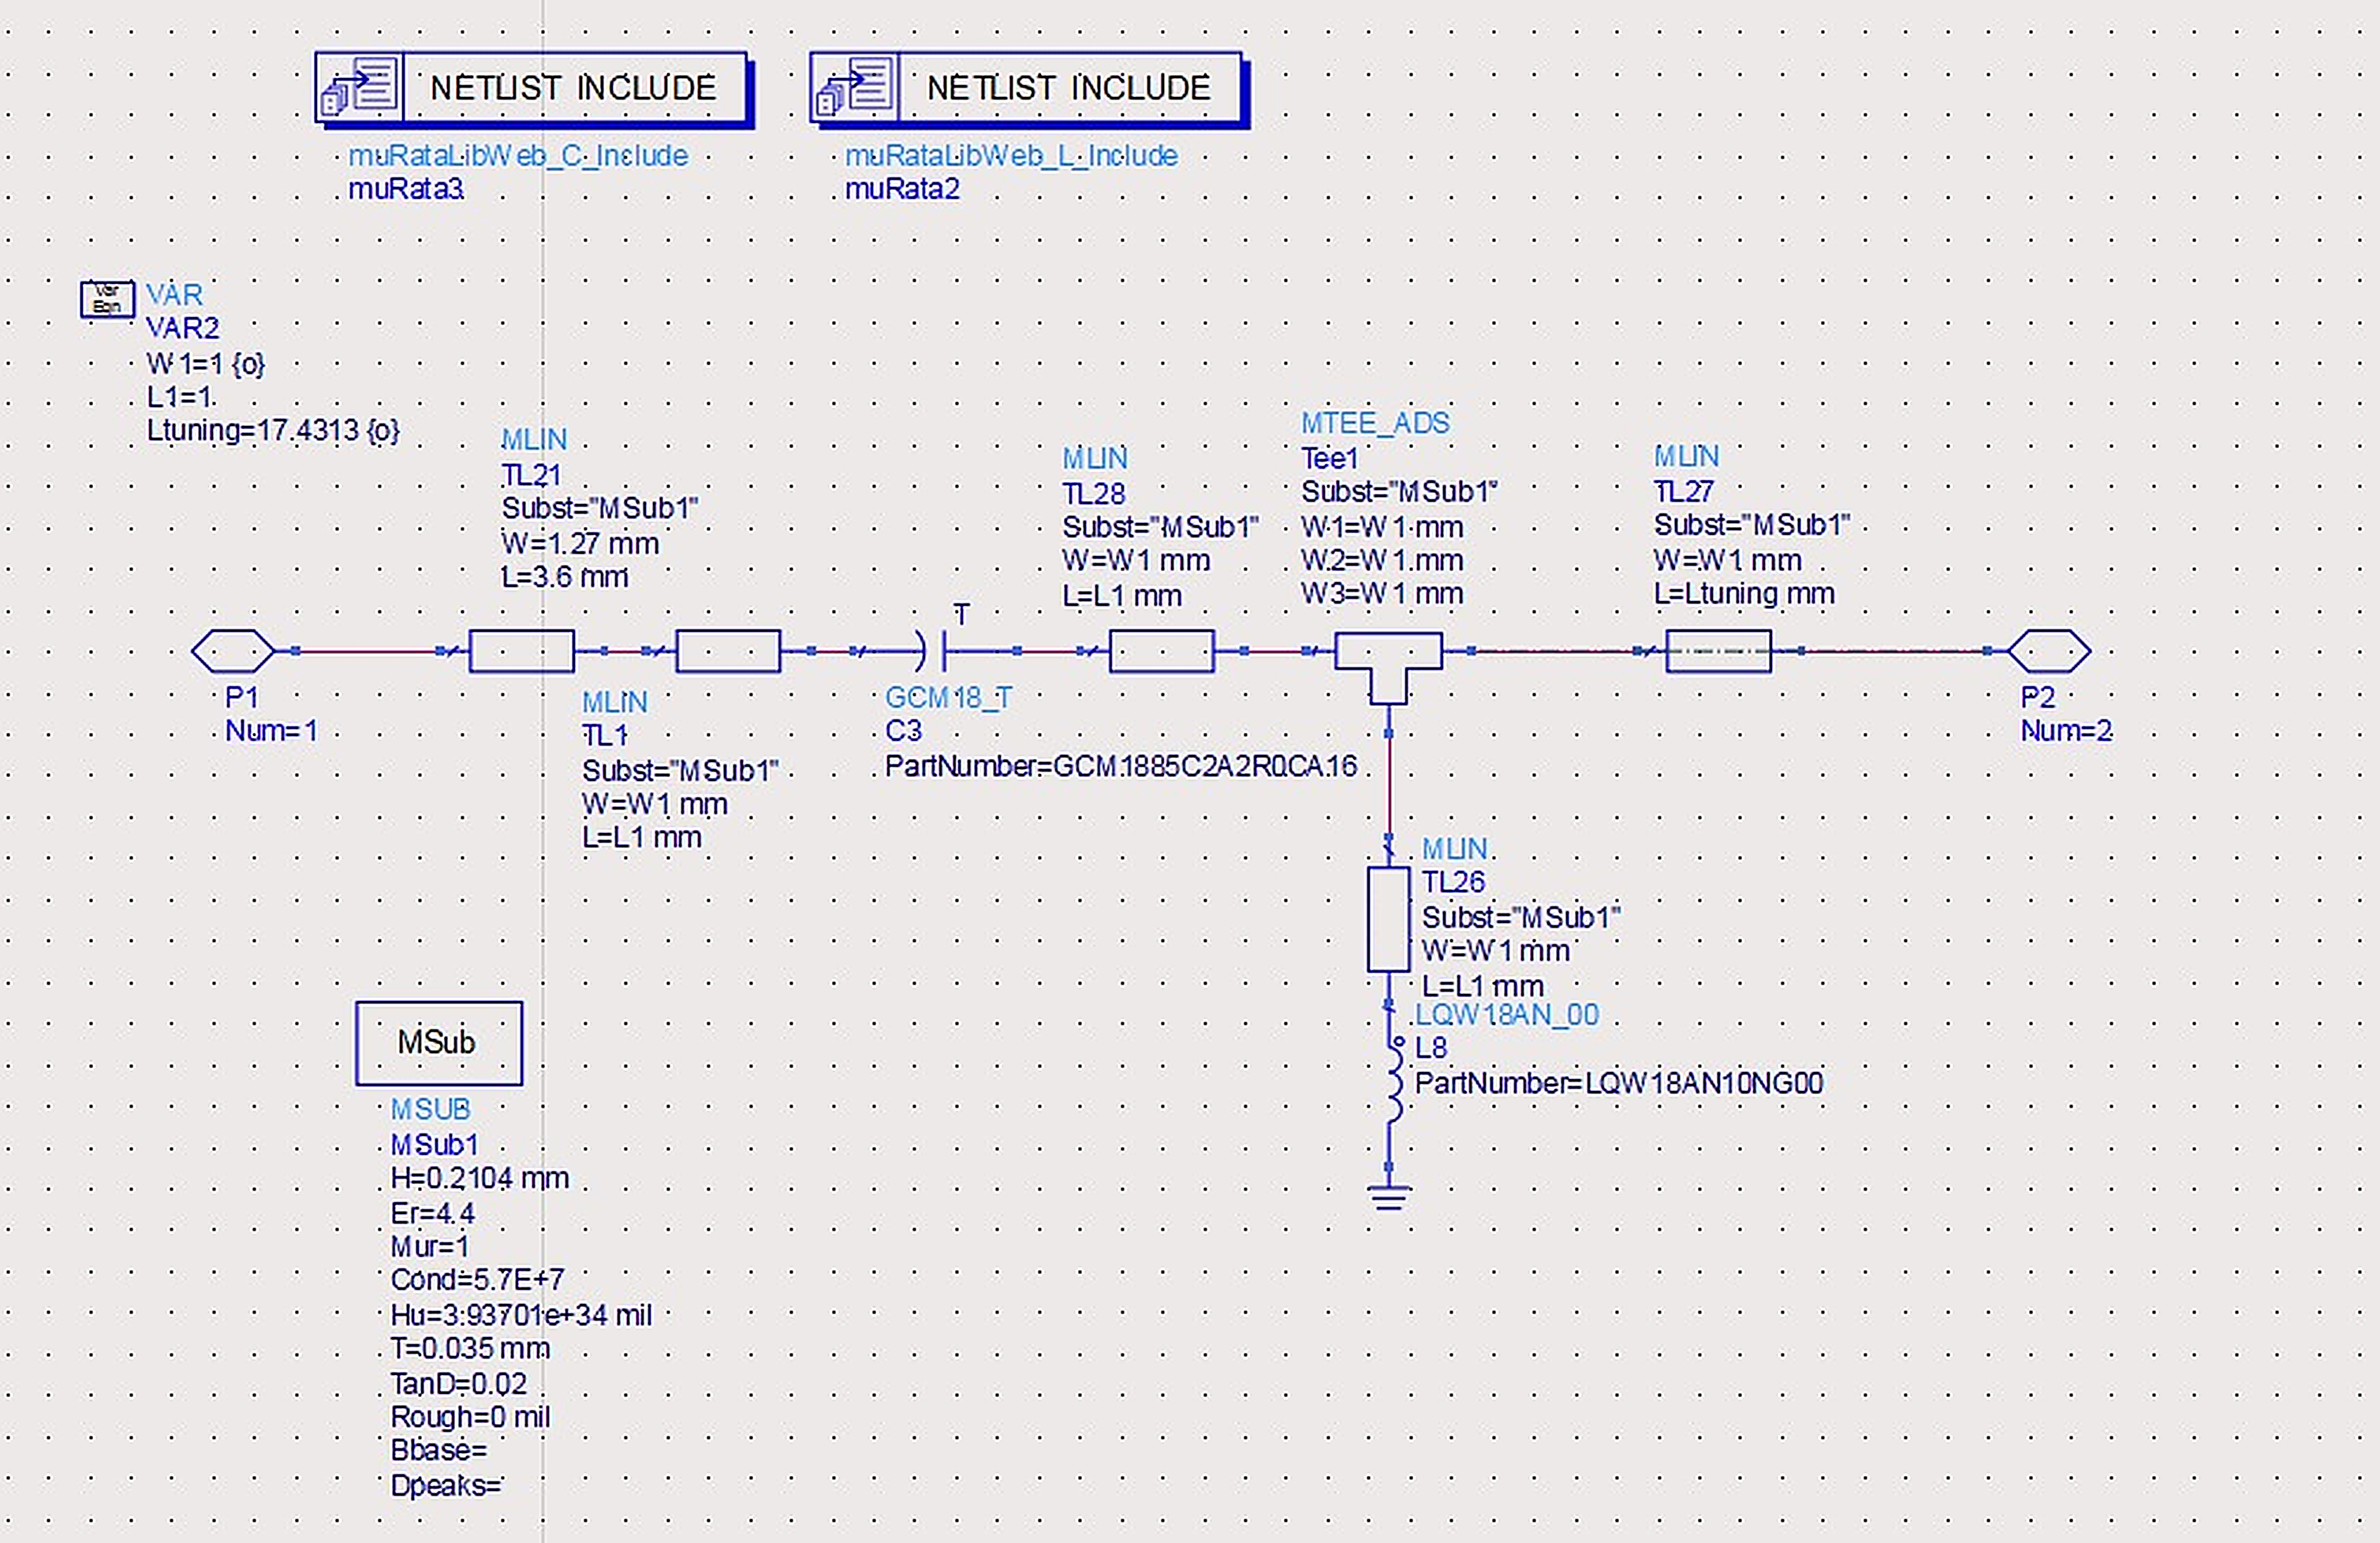
\includegraphics[width=\linewidth]{Figures/07/pa_ads_in_match.png}
    \caption{Circuito de adaptación de entrada del diseño final del amplificador de potencia.}
    \label{fig:pa_match_in}
\end{figure}

\textbf{Resultados de la optimización.} Con los componentes reales, la red de estabilidad definitiva y las redes de adaptación incorporadas, se ejecutó una nueva rutina de optimización sobre el esquemático completo, de la cual se obtuvieron los parámetros de dispersión, el contenido armónico a la salida y los parámetros de gran señal del amplificador para una potencia de entrada de 20~dBm y una tensión de alimentación de drain de 28~V.

\begin{figure}[H]
    \centering
    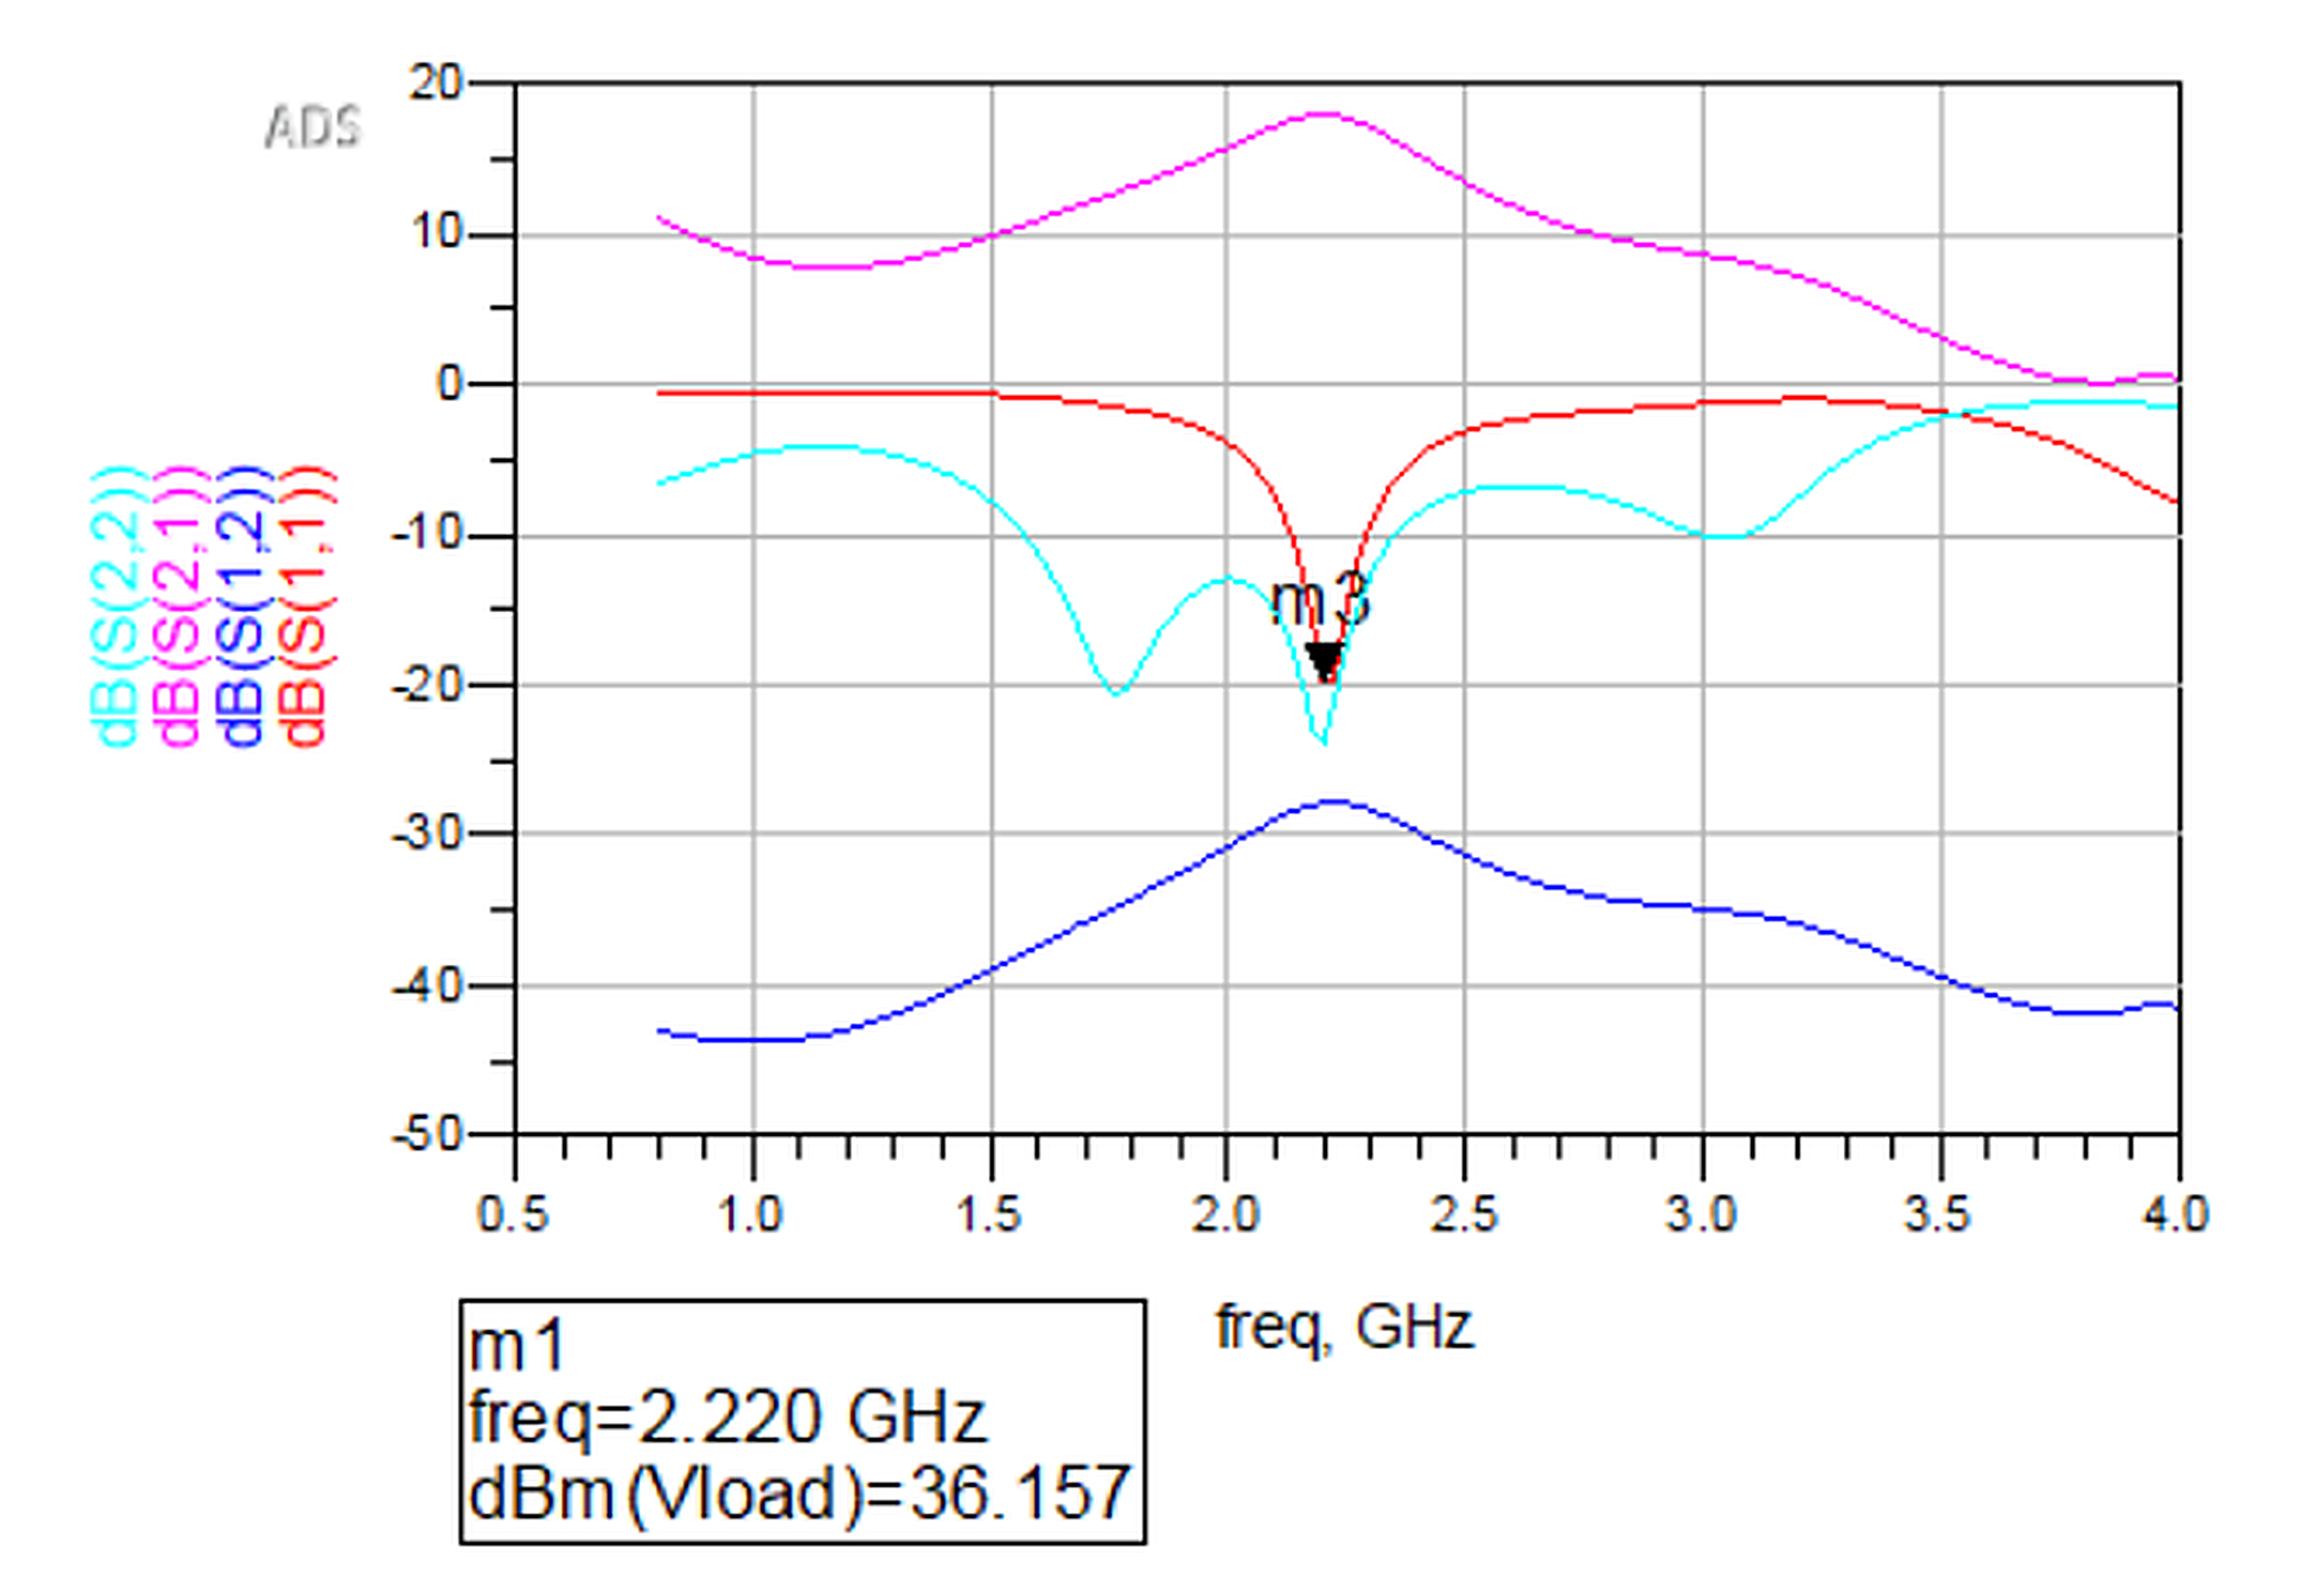
\includegraphics[width=0.75\linewidth]{Figures/07/pa_ads_sparams.png}
    \caption{Parámetros de dispersión simulados del amplificador en ADS (Pin=20\,dBm, Vdd=28\,V).}
    \label{fig:pa_ads_sparam}
\end{figure}

\begin{figure}[H]
    \centering
    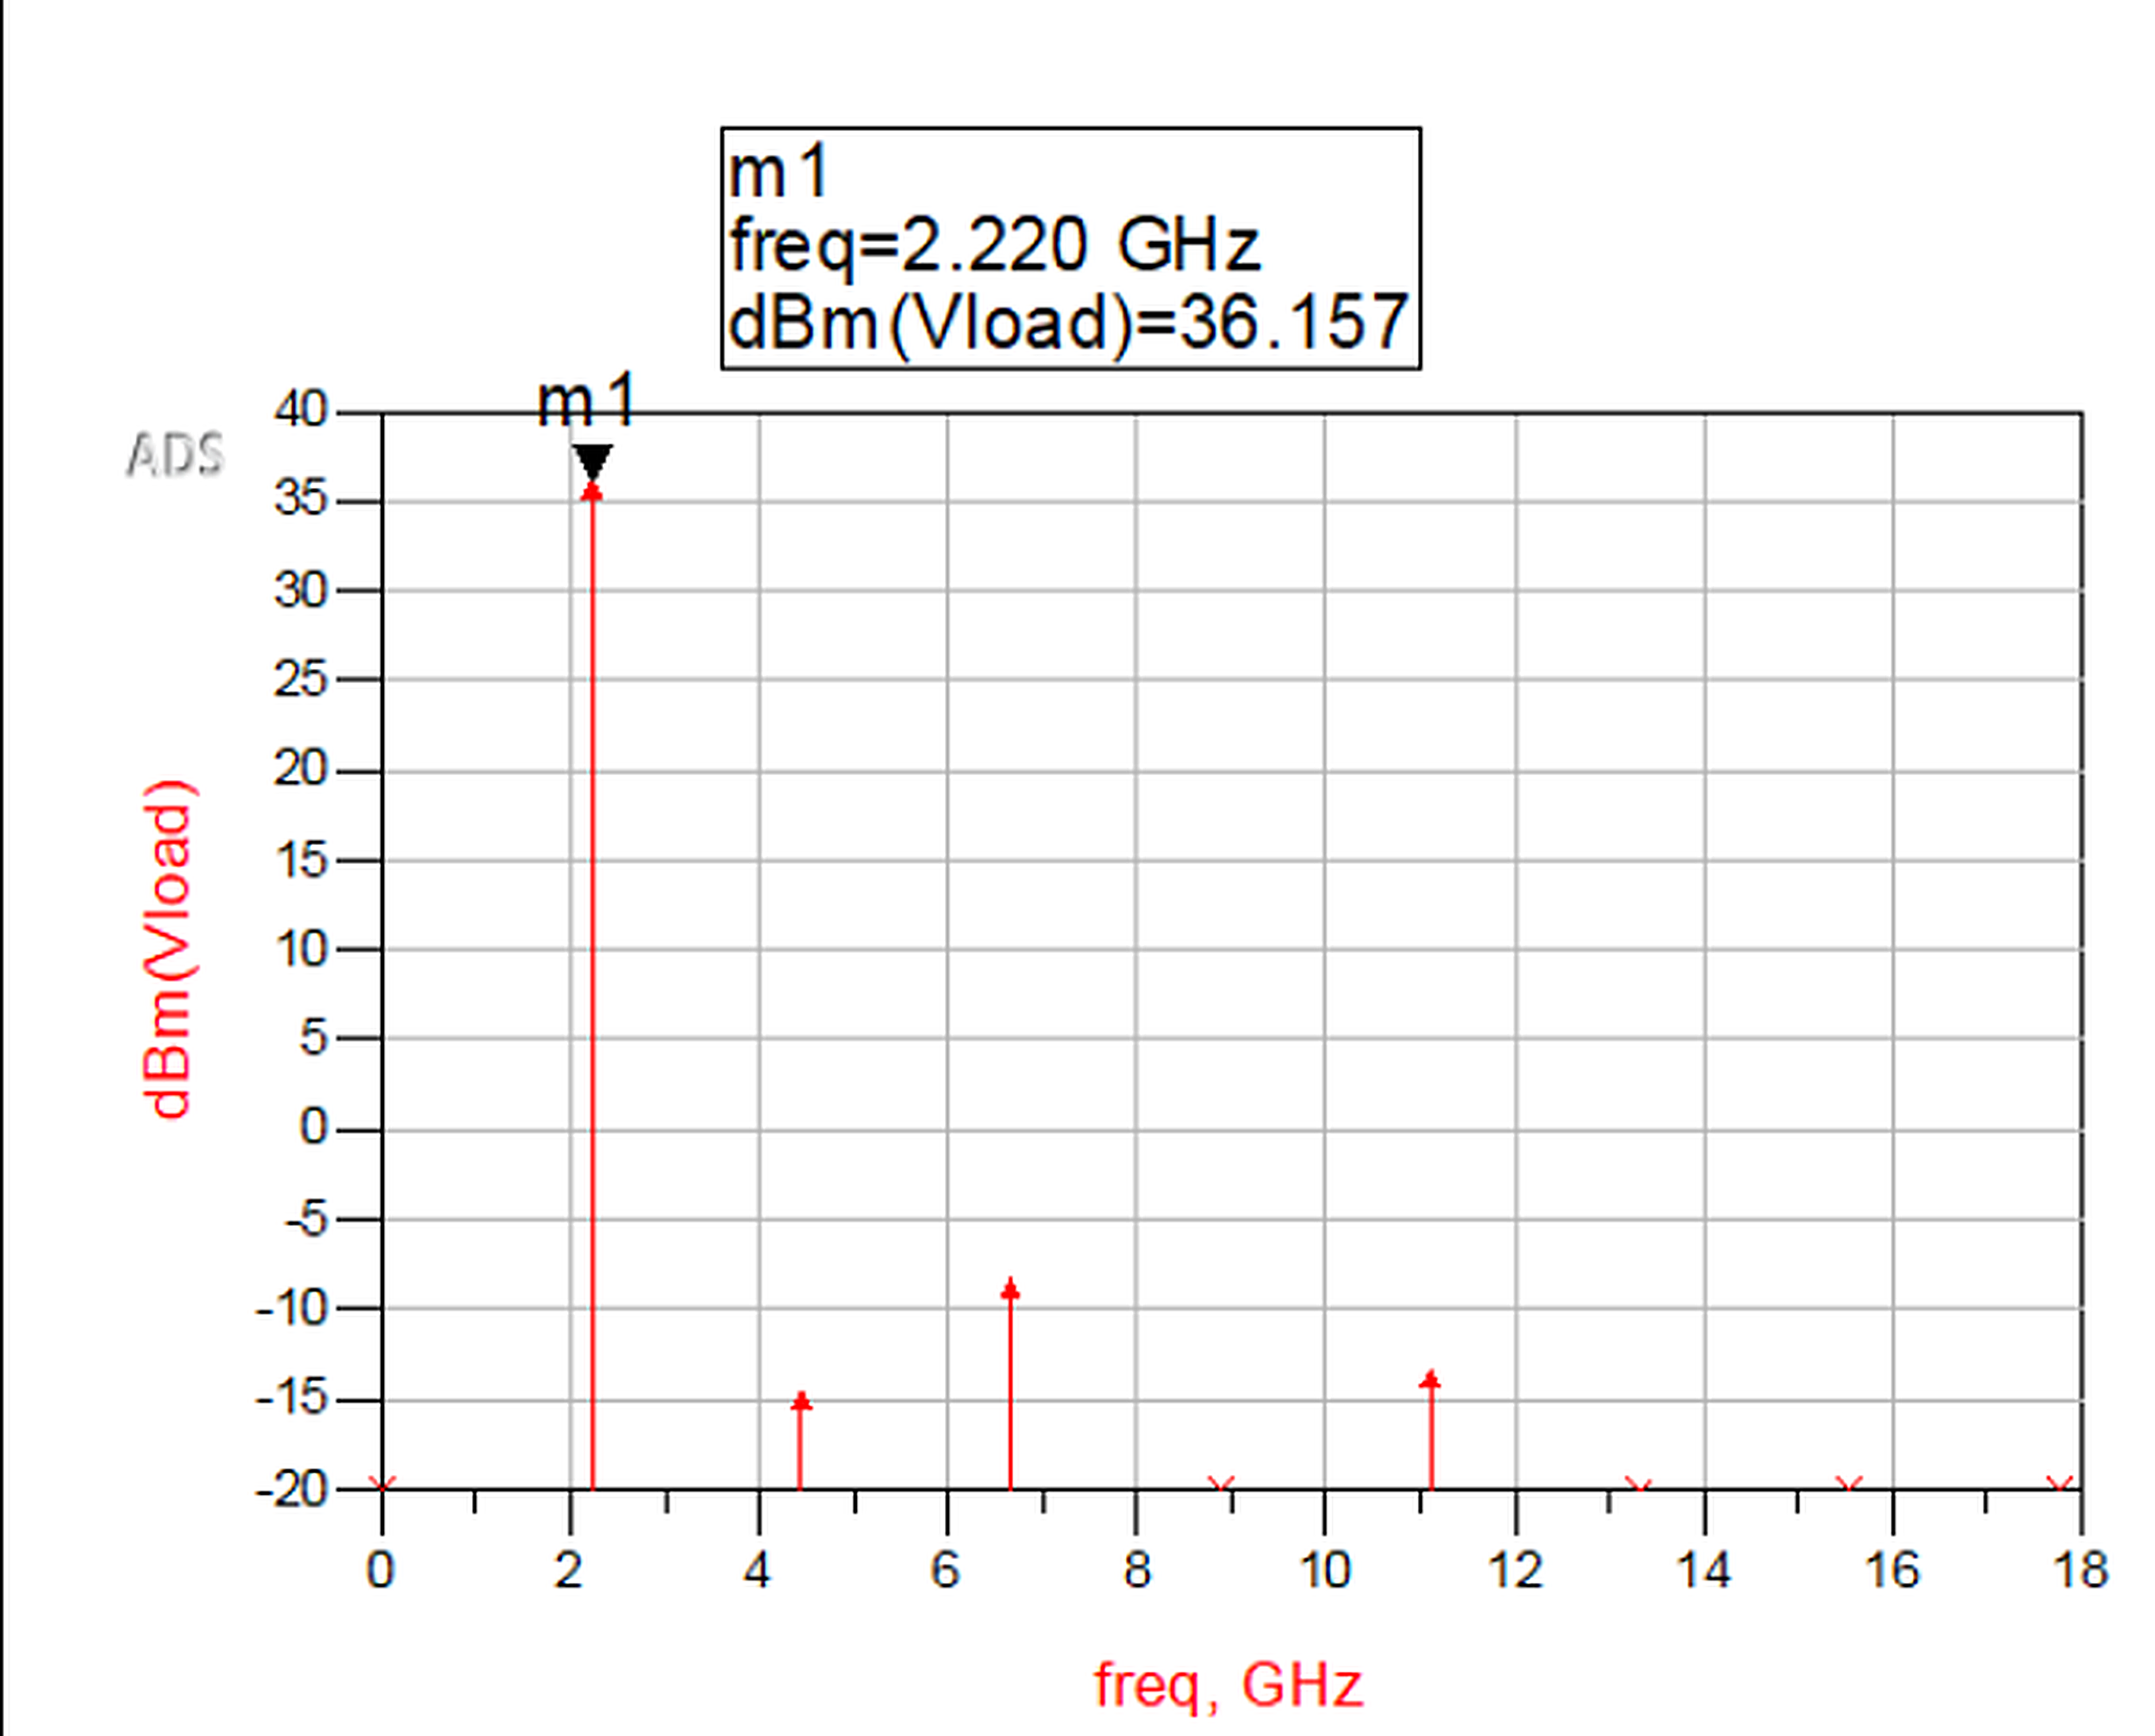
\includegraphics[width=0.7\linewidth]{Figures/07/pa_ads_harmonics.png}
    \caption{Contenido armónico simulado en la carga del amplificador (Pin=20\,dBm, Vdd=28\,V).}
    \label{fig:pa_ads_armonicos}
\end{figure}

\begin{table}[H]
    \centering
    \caption{Valores de desempeño simulados en ADS (Pin=20\,dBm, Vdd=28\,V).}
    \label{tab:pa_valores_importantes_ads}
    \begin{tabular}{lcc}
        \hline\hline
        \textbf{Parámetro}   & \textbf{Valor}  & \textbf{Unidad} \\
        \hline
        $P_{out}$            & 36,157          & dBm             \\
        Ganancia             & 16,157          & dB              \\
        PAE                  & 50,910          & \%              \\
        Eficiencia de drain  & 52,149          & \%              \\
        \hline\hline
    \end{tabular}
\end{table}

Los resultados obtenidos a nivel esquemático se consideraron satisfactorios respecto de los objetivos de diseño del Cuadro~\ref{tab:objetivos_diseno}, por lo que se procedió hacia la etapa de diseño físico del circuito impreso.

\subsection{Diseño de PCB}

\subsection{Verificación electromagnética}

% -----------------------------------------------------------------------------------------------%
\subsection{Radioenlace satelital} \label{sec:radioenlace}
Una vez determinada la potencia de salida alcanzable por el amplificador desarrollado, se realizó un análisis de radioenlace satelital o \textit{link budget}, herramienta analítica que permite cuantificar la potencia de la señal a lo largo de todo el trayecto de transmisión y comparar el nivel de señal recibido contra el umbral mínimo necesario para satisfacer la tasa de error de bit (\textit{bit error rate}, BER) requerida por la misión. El objetivo de este análisis fue determinar, a partir de la potencia de salida obtenida, qué esquemas de modulación M-PSK resultan viables para el enlace y bajo qué condiciones de elevación de la antena terrena, cerrando de esta manera el ciclo de diseño entre el desempeño real del hardware desarrollado y los requisitos de la misión.

El análisis se fundamenta en la evaluación de la densidad de flujo de potencia y las propiedades del medio físico de propagación, como fue propuesto por Friis \textbf{[REF. FRIIS]}: una antena transmisora que radia una potencia $P_t$ con una ganancia de directividad $G_t$ produce, a una distancia $d$, una densidad de flujo de potencia $S$ dada por:

\begin{equation}
    S = \frac{P_t G_t}{4\pi d^2} = \frac{\text{EIRP}}{4\pi d^2}
    \label{eq:densidad_flujo}
\end{equation}

donde EIRP representa la potencia isotrópica radiada equivalente y constituye, en términos del receptor, una cantidad equivalente a la de una fuente isotrópica ideal que produce la misma densidad de flujo en la dirección considerada. En un escenario real, la potencia entregada a la antena se ve degradada por las pérdidas mecánicas y dieléctricas en las líneas de transmisión intermedias entre el amplificador de potencia desarrollado y el puerto de alimentación de la antena, de modo que, expresado logarítmicamente, el EIRP se calcula como:

\begin{equation}
    \text{EIRP [dBW]} = P_t \text{ [dBW]} - L_{tx} \text{ [dB]} + G_{tx} \text{ [dBi]}
    \label{eq:eirp_analitico}
\end{equation}

aquí $L_{tx}$ representa las pérdidas de conducción del transmisor y $G_{tx}$ la ganancia de la antena del satélite. La potencia captada por el receptor, en este caso la estación terrena, depende de la apertura efectiva de su antena receptora ($A_e$), la cual está intrínsecamente ligada a su ganancia de directividad $G_{rx}$ y a la longitud de onda de la portadora $\lambda$ mediante la relación geométrica:

\begin{equation}
    A_e = \frac{G_{rx}\lambda^2}{4\pi}
    \label{eq:apertura_ef}
\end{equation}

de manera que la potencia disponible en los terminales del receptor ($P_r$) toma la forma de la ecuación de transferencia de Friis:

\begin{equation}
    P_r = S A_e = P_t G_t G_{rx} \left( \frac{\lambda}{4\pi d} \right)^2
    \label{eq:friis_formal}
\end{equation}

Al invertir el término entre paréntesis elevado al cuadrado en \eqref{eq:friis_formal}, se obtiene lo que se define como la pérdida de espacio libre (\textit{free space-path loss}, FSPL), magnitud que corresponde formalmente a una ganancia menor a la unidad y representa la atenuación debida a la expansión del frente de onda en el espacio sin involucrar disipación física de energía, que responde a:

\begin{equation}
    L_{FSPL} \text{ [dB]} = 20 \log_{10}\left( \frac{4\pi d}{\lambda} \right)
    \label{eq:fsl_formal}
\end{equation}

A diferencia de los enlaces terrestres fijos, la distancia $D$ en una órbita terrestre baja (LEO) es dinámicamente dependiente del ángulo de elevación de la antena ($\epsilon$) orientado hacia el satélite desde la estación terrena. Un modelo ilustrativo que ayuda a calcular esta distancia se presenta en la Figura~\ref{fig:slant_range}, donde C es el centro de la Tierra, A la posición de la antena en la superficie terrestre, S la posición del satélite en órbita a una altura $h$ y $R_E$ es el radio terrestre medio (6378~km).

\begin{figure}[H]
    \centering
    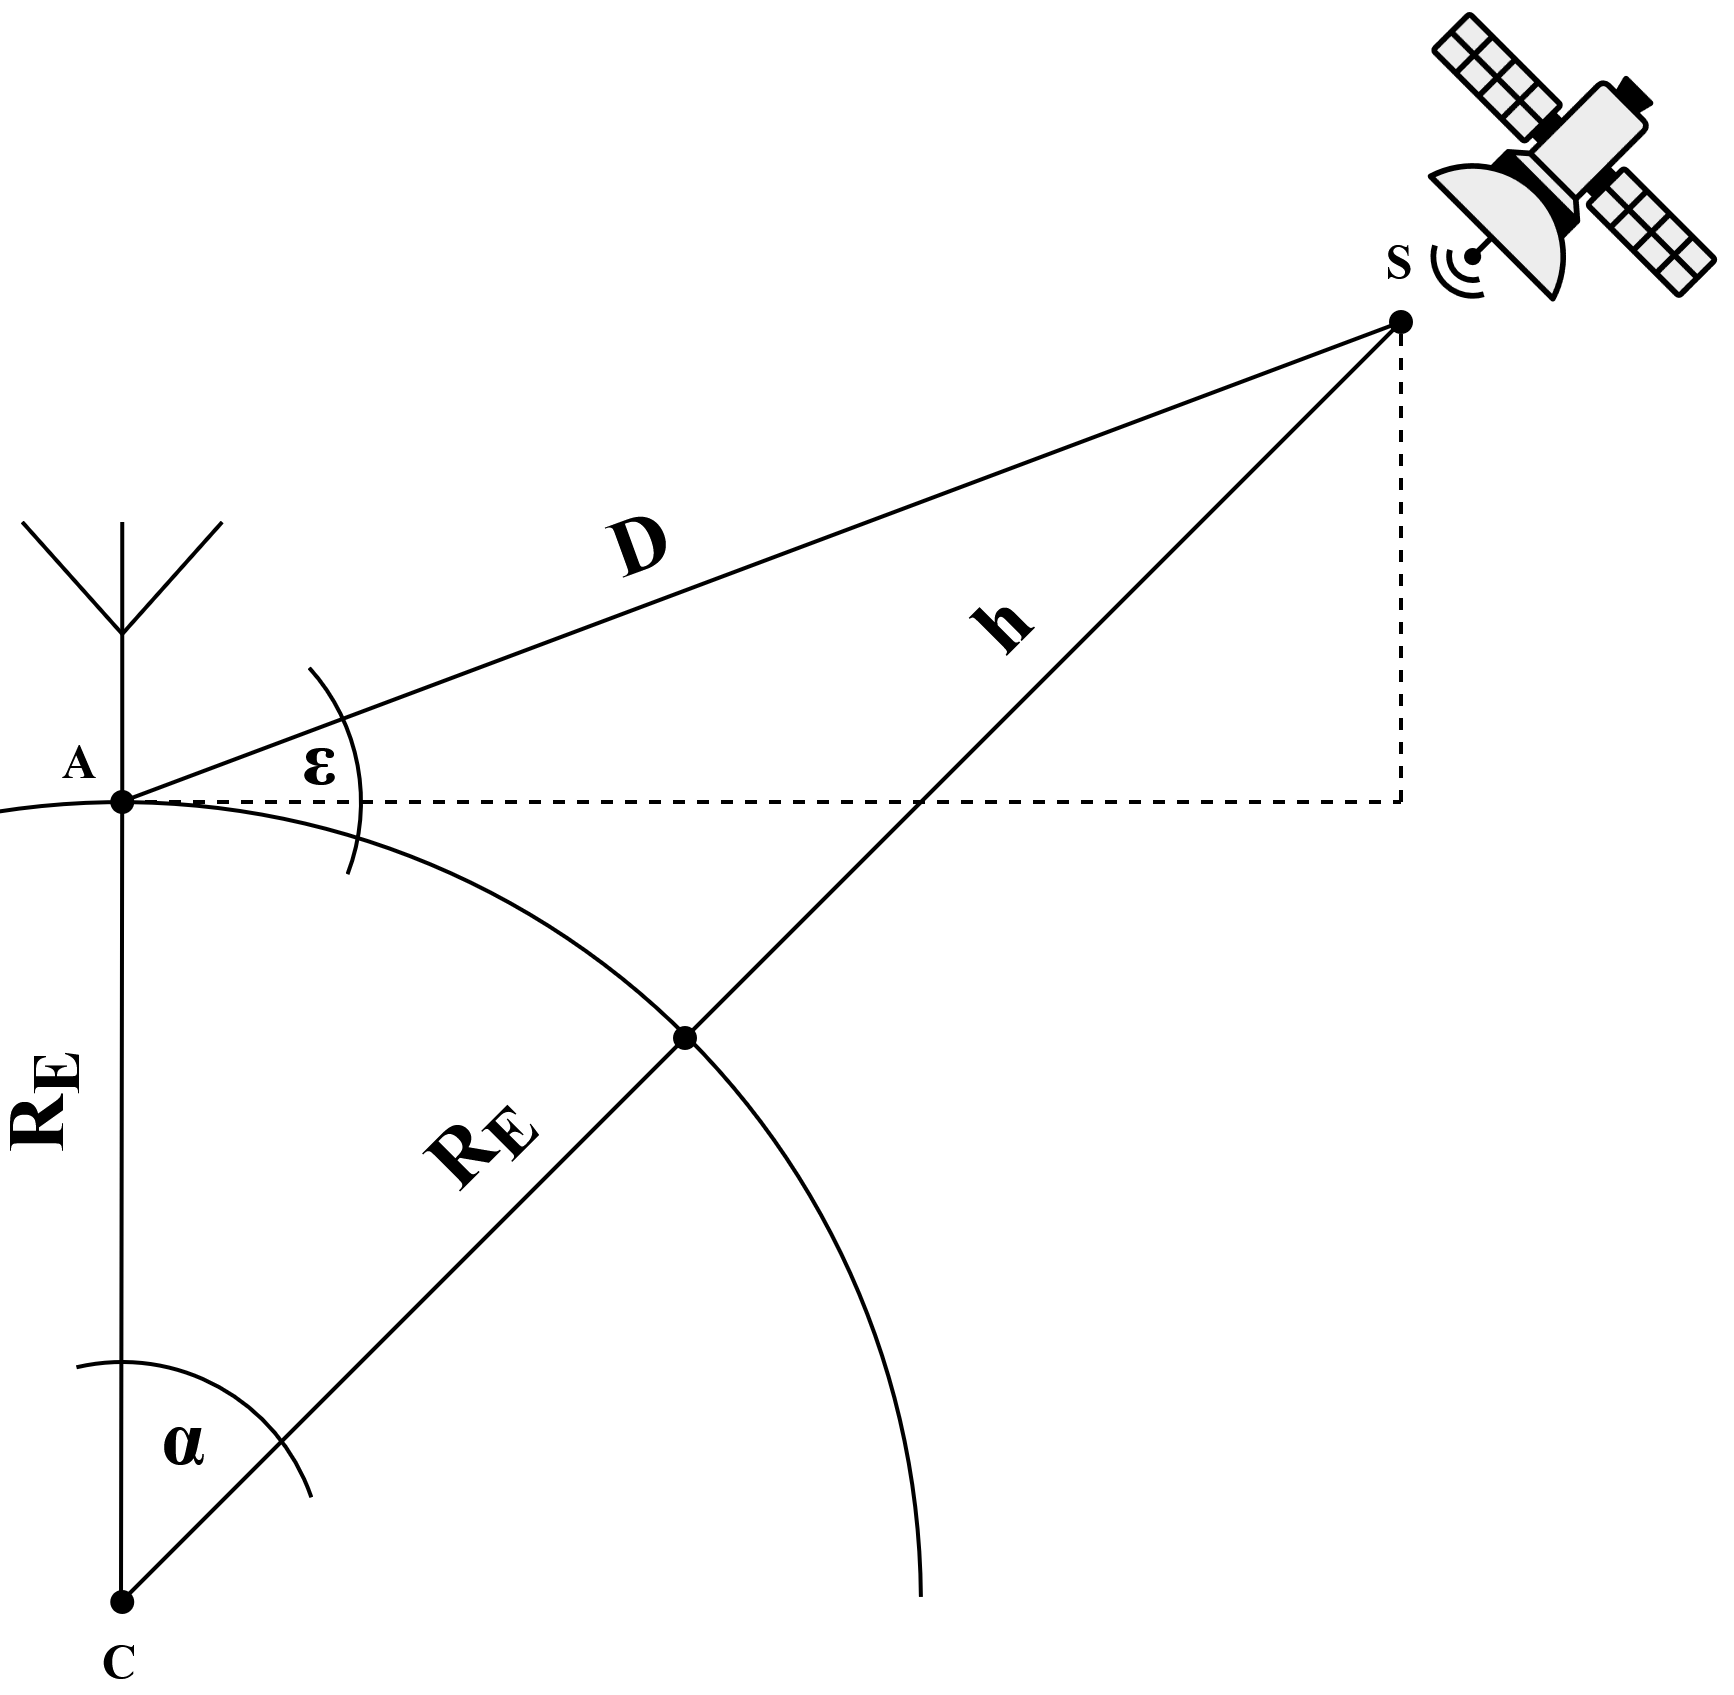
\includegraphics[width=0.7\linewidth]{Figures/07/slant_range.png}
    \caption{Modelo matemático para el cálculo de la distancia D en función del ángulo de elevación $\epsilon$.}
    \label{fig:slant_range}
\end{figure}

Utilizando la ley de los cosenos sobre la geometría esférica de la Tierra, la distancia del enlace se modela rigurosamente como:

\begin{equation}
   (R_E+h)^2 = R_E^2 + D^2 - 2\,R_E\,D\,\cos(\epsilon + \pi/2)
    \label{eq:ley_cos}
\end{equation}

Reemplazando $\cos(\epsilon+\pi/2)$ por $-\text{sen}(\epsilon)$, luego resolviendo la ecuación cuadrática para la variable $D$ y operando matemáticamente se obtiene la expresión:

\begin{equation}
    D(\epsilon) = \sqrt{(R_E + h)^2 - (R_E \cos\epsilon)^2} - R_E \sin\epsilon
    \label{eq:geometria_orbita}
\end{equation}

Como las pérdidas de espacio libre no contemplan efectos disipativos, se deben incluir en el balance de potencias las pérdidas debidas a la atmósfera y las deficiencias mecánicas de apuntamiento de las antenas, factores que, a diferencia de la FSPL, corresponden a pérdidas resistivas reales del trayecto y que se consolidan en la pérdida total de trayecto ($L_{path}$):

\begin{equation}
    L_{path}(\epsilon) \text{ [dB]} = L_{FSL}(\epsilon) + L_{point} + L_{atm}
    \label{eq:pérdidas_totales}
\end{equation}

Consecuentemente, el nivel de señal recibida (\textit{received signal level}, RSL) en función del ángulo de elevación, análogo a la diferencia entre el EIRP y la pérdida total de trayecto corregida por la ganancia neta de recepción, se determina mediante:

\begin{equation}
    \text{RSL}(\epsilon) \text{ [dBW]} = \text{EIRP} - L_{path}(\epsilon) + G_{rx} - L_{rx}
    \label{eq:rsl_formal}
\end{equation}

% ------------------------------------------------------------------------ %
\subsubsection{Modelado del ruido y calidad del enlace}
La viabilidad del enlace digital no se limita a la amplitud de la portadora recibida, sino a su relación respecto a la densidad espectral de potencia de ruido térmico presente en el sistema ($N_0$), modelado como ruido blanco gaussiano aditivo. En sistemas terrestres, este ruido suele caracterizarse mediante la figura de ruido del receptor referida a una temperatura estándar de 290\,K, sin embargo, en estaciones terrenas de comunicaciones satelitales la antena recibe directamente el ruido de cielo, sustancialmente menor a 290\,K, por lo cual resulta más preciso emplear una temperatura total de sistema en lugar de una figura de ruido equivalente. Bajo este criterio, la temperatura total de ruido del sistema receptor ($T_{sys}$) se descompone aditivamente de acuerdo con el teorema de uniones en cascada, simplificado para los componentes críticos del segmento terreno:

\begin{equation}
    T_{sys} = T_{ant} + T_{LNA}
    \label{eq:tsys}
\end{equation}

donde $T_{ant}$ es la temperatura de ruido equivalente de la antena, que captura la radiación de fondo cósmico y el ruido térmico terrestre captado por los lóbulos secundarios, y $T_{LNA}$ es la temperatura de ruido efectiva referida a la entrada del amplificador de bajo ruido. La densidad espectral de ruido resultante se expresa logarítmicamente como:

\begin{equation}
    N_0 \text{ [dBW/Hz]} = k_{dB} + 10 \log_{10}(T_{sys})
    \label{eq:n0_log}
\end{equation}

% TODO: se omitieron las ecuaciones eb/n0 (eq:ebn0_rb y eq:ebn0_bw) presentes en el
% archivo original entre esta ecuación y la siguiente, deben reincorporarse tal
% como estaban en 07-2-Radioenlace.tex al integrar este archivo al documento final.

donde el único parámetro de la cadena de transmisión digital que interviene en la ecuación es la tasa de bits $R_b$, con independencia de cómo esta haya sido determinada. En sistemas con asignación espectral rígida, $R_b$ no constituye un parámetro libre sino una cantidad derivada del ancho de banda ocupado ($BW$) y de las características del esquema de modulación. La tasa de símbolos (\textit{symbol rate}, $R_s$) en baudios se deduce a partir del factor de roll-off $\alpha$ del filtro de coseno realzado empleado para conformar el espectro, dado que la relación entre el ancho de banda ocupado y la tasa de símbolos para este tipo de filtrado responde a:

\begin{equation}
    R_s = \frac{BW}{1 + \alpha}
    \label{eq:rs_bw}
\end{equation}

A partir de la eficiencia espectral del esquema de modulación lineal M-PSK implementado, la tasa de bits efectiva queda determinada por la cantidad de bits por símbolo ($\log_{2}M$):

\begin{equation}
    R_b = R_s \log_{2}(M) = \frac{BW}{1 + \alpha} \log_{2}(M)
    \label{eq:rb_deducido}
\end{equation}

de modo que, bajo un ancho de banda constante, el aumento en el orden de la modulación $M$ incrementa la tasa de transmisión a costa de una reducción proporcional en el $E_b/N_0$ disponible por bit, según se desprende de sustituir \eqref{eq:rb_deducido} en la expresión de $E_b/N_0$ en función de $R_b$.

El valor de $[E_b/N_0]_{req}$ que interviene en el criterio de cierre del enlace no es un parámetro arbitrario, sino que depende exclusivamente de dos factores: el esquema de modulación digital empleado y la tasa de error de bit (BER) objetivo de la misión. Esta dependencia se establece a través de la función de error complementaria gaussiana, comúnmente expresada mediante la función $Q(z)$, que es la herramienta analítica para poder vincular la relación señal a ruido disponible con la probabilidad de error de detección en presencia de ruido.

\begin{equation}
    Q(z) = \frac{2}{\sqrt{\pi}} \int_{z}^{\infty} e^{-t^2}\, dt
    \label{eq:funcion_q}
\end{equation}

Para un esquema de modulación M-PSK, sujeto a detección coherente sobre un canal AWGN, la tasa de error de bit puede aproximarse en función de $E_b/N_0$ mediante:

\begin{equation}
    \text{BER} \approx \frac{2}{\log_{2}(M)}\, Q\!\left( \sqrt{2 \log_{2}(M)} \, \sin\!\left(\frac{\pi}{M}\right) \sqrt{\frac{E_b}{N_0}} \right)
    \label{eq:ber_mpsk}
\end{equation}

expresión que, al ser invertida numéricamente para una BER objetivo preestablecida, permite obtener el valor de $[E_b/N_0]_{req}$ correspondiente a cada orden de modulación $M$. De esta manera, modulaciones de mayor orden, que ofrecen una mayor eficiencia espectral al transmitir más bits por símbolo, exigen simultáneamente una relación $E_b/N_0$ más elevada para sostener la misma tasa de error, lo cual constituye el compromiso fundamental entre velocidad de transmisión y robustez frente al ruido que se evalúa a lo largo de este balance de enlace.

Para asegurar la robustez del enlace ante desvanecimientos repentinos o imprecisiones, el margen operativo instantáneo $M_{arg}(\epsilon)$ frente al requerimiento teórico de la modulación empleada ($[E_b/N_0]_{req}$) debe superar un umbral mínimo preestablecido ($M_{min}$):

\begin{equation}
    M_{arg}(\epsilon) = \frac{E_b}{N_0}(\epsilon) - [E_b/N_0]_{req} \ge M_{min}
    \label{eq:margen}
\end{equation}

El cumplimiento de esta desigualdad define analíticamente el ángulo de elevación mínimo de visibilidad operativa $\epsilon_{min}$, por debajo del cual el enlace se considera no viable para la comunicación con la modulación correspondiente.

% ------------------------------------------------------------------------ %
\subsubsection{Implementación computacional y simulación}
Con el propósito de validar los rangos de operación del amplificador de potencia diseñado y determinar los límites físicos de la comunicación, se desarrollaron dos herramientas en lenguaje Python que implementan las ecuaciones~\eqref{eq:eirp_analitico} a \eqref{eq:margen}, utilizando interfaces gráficas interactivas basadas en la biblioteca \textit{Tkinter} e integración de cálculo numérico vectorizado con \textit{NumPy} y visualización mediante \textit{Matplotlib}.

El primer programa desarrollado (\texttt{link\_budget.py}) evalúa la viabilidad del enlace fijando una tasa de bits (\textit{bit rate}) analítica única y configurable para todo el sistema. El \textit{script} barre el vector de ángulos de elevación $\epsilon \in [0^\circ, 90^\circ]$ y calcula una única curva de $E_b/N_0$ disponible en función de la elevación. Dado que la tasa de bits es común a todo el sistema, esta misma curva se contrasta simultáneamente contra los tres umbrales requeridos ($[E_b/N_0]_{req}$ de QPSK, 8-PSK y 16-PSK), determinando para cada modulación el primer índice angular que satisface el criterio de cierre de la ecuación~\eqref{eq:margen}.

El segundo programa (\texttt{link\_budget\_bw.py}) refina el análisis adaptándolo a las limitaciones físicas de canalización del transceptor. Este algoritmo toma como variables de entrada el ancho de banda ocupado en radiofrecuencia ($BW$) y el factor de roll-off del filtro ($\alpha$), a partir de los cuales calcula una tasa de símbolos común mediante la ecuación~\eqref{eq:rs_bw} y, posteriormente, deriva una tasa de bits específica para cada esquema de modulación multiplicando dicha tasa de símbolos por la cantidad de bits por símbolo correspondiente (2 para QPSK, 3 para 8-PSK y 4 para 16-PSK), de acuerdo con la ecuación~\eqref{eq:rb_deducido}. A diferencia del primer \textit{script}, en este caso cada modulación posee su propia tasa de bits efectiva y, en consecuencia, su propia curva de $E_b/N_0$ disponible en función de la elevación, calculada de forma independiente; el resultado son tres curvas diferenciadas, y no una curva única contrastada contra tres umbrales, lo cual modela fielmente el compromiso entre el orden de la modulación, la velocidad de transmisión resultante y la degradación del margen disponible frente al ruido térmico.

Los parámetros de simulación nominales cargados por defecto en ambas herramientas informáticas, representativos de la arquitectura física del CubeSat y el segmento terreno en banda S, se consolidan en el Cuadro~\ref{tab:parametros_scripts}.

\begin{table}[H]
    \centering
    \caption{Parámetros de diseño y simulación empleados en los scripts de cálculo de radioenlace.}
    \label{tab:parametros_scripts}
    \begin{tabular}{lccc}
        \hline\hline
        \textbf{Parámetro del Sistema}             & \textbf{Símbolo} & \textbf{Valor}  & \textbf{Unidad} \\
        \hline
        Frecuencia de Operación                    & $f$              & 2,2             & GHz  \\
        Radio de la Órbita Satelital               & $h_{orb}$        & 600             & km   \\
        Ancho de Banda de Canal                    & $BW$             & 10,0            & MHz  \\
        Factor de Roll-off del Filtro              & $\alpha$         & 0,35            & ---  \\
        Tasa de Bits de Referencia                 & $R_b$            & 500             & kbps \\
        Potencia de Salida del Transmisor          & $P_t$            & 0,0             & dBW  \\
        Pérdidas en la Línea del Transmisor        & $L_{tx}$         & 1,0             & dB   \\
        Ganancia de la Antena Transmisora          & $G_{tx}$         & 5,0             & dBi  \\
        Pérdidas por Apuntamiento de Antena        & $L_{point}$      & 1,0             & dB   \\
        Pérdidas por Atenuación Atmosférica        & $L_{atm}$        & 1,0             & dB   \\
        Ganancia de la Antena Receptora            & $G_{rx}$         & 25,0            & dBi  \\
        Pérdidas en el Sistema Receptor            & $L_{rx}$         & 1,0             & dB   \\
        Temperatura de Antena                      & $T_{ant}$        & 55              & K    \\
        Temperatura de Ruido del LNA               & $T_{LNA}$        & 120             & K    \\
        Margen Establecido                         & $M_{min}$        & 1,0             & dB   \\
        \hline\hline
    \end{tabular}
\end{table}

A continuación, las Figuras~\ref{fig:grafico_bitrate} y \ref{fig:grafico_bw} ilustran las curvas de desempeño obtenidas mediante las interfaces gráficas implementadas para cada una de las metodologías analizadas.

\begin{figure}[H]
    \centering
    % \includegraphics[width=0.8\linewidth]{Figures/07/grafico_bitrate.png}
    \caption{Curva de $E_b/N_0$ disponible frente a elevación para una tasa de bits constante ($R_b = 500\text{ kbps}$) generada por el script \texttt{link\_budget.py}.}
    \label{fig:grafico_bitrate}
\end{figure}

\begin{figure}[H]
    \centering
    % \includegraphics[width=0.8\linewidth]{Figures/07/grafico_bw.png}
    \caption{Curvas diferenciadas de $E_b/N_0$ disponible por modulación para un ancho de banda fijo ($BW = 10\text{ MHz}$) generadas por el script \texttt{link\_budget\_bw.py}.}
    \label{fig:grafico_bw}
\end{figure}